%% Electro-optic study of AlGaAs coated mirrors

 As mentioned in Section \cite{sec:ligo_noise} one of the many LIGO fundamental noise sources is coating thermal noise from the $\mathrm{SiO_2}/\mathrm{TiO_2:Ta_2O_5}$ aLIGO coatings. As aLIGO approaches its designed sensitivity various coating solutions are currently proposed to mitigate thermal noise coupling into the detector output \cite{?}. With the potential to reduce coating Brownian noise by a factor of 10 \cite{Cole:2013}, $\gaas$/$\algaas$ shows much promise with next generation detectors for a potential strain reduction by a factor of 5 \cite{?}, in comparison to the current aLIGO coatings. Though inherent material property differences of these crystalline coatings introduce new and potentially significant noise couplings; one being the linear electro-optic property of crystalline materials (dn/dE), also known as the Pockels effect \cite{abernathy_poster}. Prior to commitment of a $\gaas$/$\algaas$ coating in gravitational wave detectors, a thorough study of these notable noises is worthwhile. This section details a study of starting with a survey of the distinguishing optical and material properties of crystalline materials like $\gaas$ and $\algaas$ by reviewing: light propogation through anistropic materials, and induced optical anisotropy of zincblende materials. Immediately after, estimates of the differential phase of light reflected from a $\gaas$/$\algaas$ coating caused by electric field noise are computed with potential impacts to current generation gravitational wave detectors. With adequate motivation, an experiment designed to measure the pockels effect from a HR $\gaas$/$\algaas$ coated ``witness" sample was constructed and the design, results are discussed.

\subsection{Anisotropic media}
Unlike with isotropic media, we cannot assume that the index of refraction of anisotropic media is the same for all chosen wave vectors. This is a direct consequence of the birefringence of anisotropic media; characterized by the dielectric, permittivity, and polarization tensors.

\subsubsection{The Dielectric tensor}
Further elaborating on the nature of a generalized dielectric tensor for any wavevector is required to proceed:
\begin{equation}\label{eq:3.11}
D_i = \varepsilon_{ij}E_j
\end{equation}
Where D is the displacement vector and E is the electric field vector and $\varepsilon$ is the dielectric tensor. The displacement vector for isotropic media is retrieved when $i = j$ and $\varepsilon_i = \varepsilon$. To further understand the nature of the dielectric tensor we assert Poynting's theorem providing an energy conservation requirement:
\begin{equation}\label{eq:3.12}
\nabla \cdot \vec{S} = \frac{dU}{dt}
\end{equation}
Where $\vec{S} = \vec{E} \times \vec{H}$ is the poynting vector and $U = \frac{1}{8 \pi} \big( \vec{E} \cdot \vec{D} + \vec{B} \cdot \vec{H} \big)$ is the electromagnetic field density. The reader is left to perform the exercise and show that in order for \ref{eq:3.12} to hold true given \ref{eq:3.11}


\begin{equation}
\varepsilon_{ij} = \varepsilon_{ji}
\end{equation}
Demonstrating that the dielectric tensor is symmetric - exhibiting only six unique terms. Diagonalizing the tensor, the presence of two unique eigenvectors and eigenvalues indicates the existance of two eigenpolarizations with paired eigenindices.
%The most general form of the energy density can be geometrically represented as ellipsoid but a coordinate transformation we can diagonalize and realize the principal axes of the dielectric allowing a simpler form of the displacement, and in turn the energy density.

\subsubsection{Monochromatic plane wave propogation}
Revisiting Maxwell's equations for simple monochromatic plane wave solution gives provides further direction on how crystalline media may effect incident light. Further elaborating, the following assumptions are made:
\begin{equation}
\vec{E} = E_o e^{(i \omega (\frac{n}{c} \vec{r}\cdot \vec{s}-t))}
\end{equation}
Where $n$ is the index of refraction, $c$ is the speed of light, $\vec{r}$ is the position vector and $\vec{s}$ is the unit wave normal.
\begin{equation}
\nabla \times \vec{H}= \frac{\partial \vec{D}}{\partial t}
\end{equation}
Where $\vec{H}$ is the magnetic field assuming the permeability $\mu$, and the generalized displacement vector $\vec{D}$ and electric field vector $\vec{E}$.
\begin{equation}
\nabla \times \vec{E} = -\mu \vec{H}
\end{equation}
Reducing to only the displacement and electric fields:
\begin{equation}\label{eq:3.17}
\vec{D} = \frac{n^2}{\mu}[\vec{E}-\vec{s}(\vec{s}\cdot \vec{E})]
\end{equation}
Maxwell's equations show that the electric field is not necessarily parallel to the displacement field and in most materials with non-zero polarizability tensors and dielectric tensors, it is not. But as specified above, the displacement vector, Electric field and unit wave normal are co-planar while remaining orthogonal to $\vec{H}$. Assuming we are operating within a coordinate system aligned with the principal dielectric axes, we substitute \ref{eq:3.11} into \ref{eq:3.17}:
\begin{equation}\label{eq:3.18}
E_i = \frac{n^2 s_i (\vec{E}\cdot\vec{s})}{n^2 - \mu \varepsilon_i}
\end{equation}

From here it can be shown that for a general plane wave there exist two unique refractive index solutions within the constructed dielectric. Though using this result to show this requires revisiting geometrical conditions that are best visualized using a method introduced in the next section. \textcolor{red}{For a more rigorous proof, see Appendix H in} \cite{nye}

\subsubsection{Indicatrix}\label{sec:indicatrix}
Acquiring solutions of the two indices along with the corresponding directions of propogation in the crystal for a general plane wave with unit wave vector $\vec{s}$ can be done via a conveniant geometrical construction. The construction begins by considering a constant electric energy density ($U_e$) surface in the $\vec{D}$ space; an ellipsoid is formed:

\begin{equation}\label{eq:lagr1}
\frac{D_x}{\varepsilon_x} + \frac{D_y}{\varepsilon_y} + \frac{D_z}{\varepsilon_z} = 2 U_e \varepsilon_o
\end{equation}
With redefined coordinates $(\vec{D}/\sqrt{2 U_e \varepsilon_o}) \rightarrow \vec{r}$ and setting $\varepsilon_i = n^2_i$:
\begin{equation}
\frac{x^2}{n_x^2} + \frac{y^2}{n_y^2} + \frac{z^2}{n_z^2} = 1
\end{equation}
This equation for the ellipsoid is known as the indicatrix. Given the co-planar solution demonstrated in the last section, we can impose the normal of the plane $\vec{r} \cdot \vec{s} = 0$:

\begin{equation}\label{eq:lagr2}
\vec{r} \cdot \vec{s} = x s_x + y s_y + z s_z = 0
\end{equation}
Equations \ref{eq:lagr1} and \ref{eq:lagr2} both contribute constraints to the method of finding extrema using Lagrange multipliers for the function:
\begin{equation}
r^2 = x^2 + y^2 + z^2
\end{equation}
The Lagrangian ($\mathcal{L}$) with the introduced multiplers ($\lambda_1$, $\lambda_2$) then becomes:
\begin{equation}
\mathcal{L}(\textcolor{red}{\vec{r},\vec{s}},\lambda_1, \lambda_2) =
x^2 + y^2 + z^2 + \lambda_1 (xs_x + ys_y + zs_z) + \lambda_2 \bigg( \frac{x^2}{\varepsilon_x} + \frac{y^2}{\varepsilon_y} + \frac{z^2}{\varepsilon_z} - 1 \bigg)
\end{equation}
With the generated system of equations from the Lagrange multipler method ($\partial F_i/ \partial x_i = 0$, and $\partial F_j/ \partial \lambda_j$) where index $i =x,y,z$ and $j = 1,2$ we obtain a system of 3 equations:
\begin{equation}
i \bigg(1-\frac{r^2}{\varepsilon_{i}} \bigg) + s_{i} \bigg(\frac{x s_x}{\varepsilon_x} + \frac{y s_y}{\varepsilon_y} + \frac{z s_z}{\varepsilon_z} \bigg) = 0
\end{equation}
The result is verified when substituting $r \rightarrow \frac{\vec{D}}{\sqrt{\vec{E} \cdot \vec{D} \varepsilon_o}}$ back which recovers \ref{eq:3.18}.
\\

\begin{figure}[H]
\begin{center}
\includegraphics[width=75mm]{figs/ALGAAS/indicatrix_nye.pdf}
\end{center}
\caption{General ellipsoid indicatrix with a general propogation direction (Using Nye's figure as placeholder as of now)}
\label{fig:general_indicatrix}
\end{figure}

\subsection{$\gaas$ and $\algaas$ crystal classification}
The space group of $\gaas$ as well as $\algaas$ are within the $F\bar{4}3m$ space group. Crystals of this particular space group are commonly known as zincblende crystals; a common crystal configuration named after zinc sulfide (ZnS). Cubic crystals by their crystallographic structure display optically isotropic characteristics when  stress free and no DC and/or slowly varying electric fields are present.
\satoshi{Is this true?} \textcolor{blue}{Yes. Though the birefringence seen from HR $\gaas$ coatings is said to be due to an ``intrinsic stress" in the high and low index layers. (What is breaking the symmetry to cause this? Heteroepitaxy? Annealing? Defects? Is this birefringence the same for all samples?) I think a dedicated high precision birefringence measurement on multiple samples would be cool.}

\begin{figure}[H]
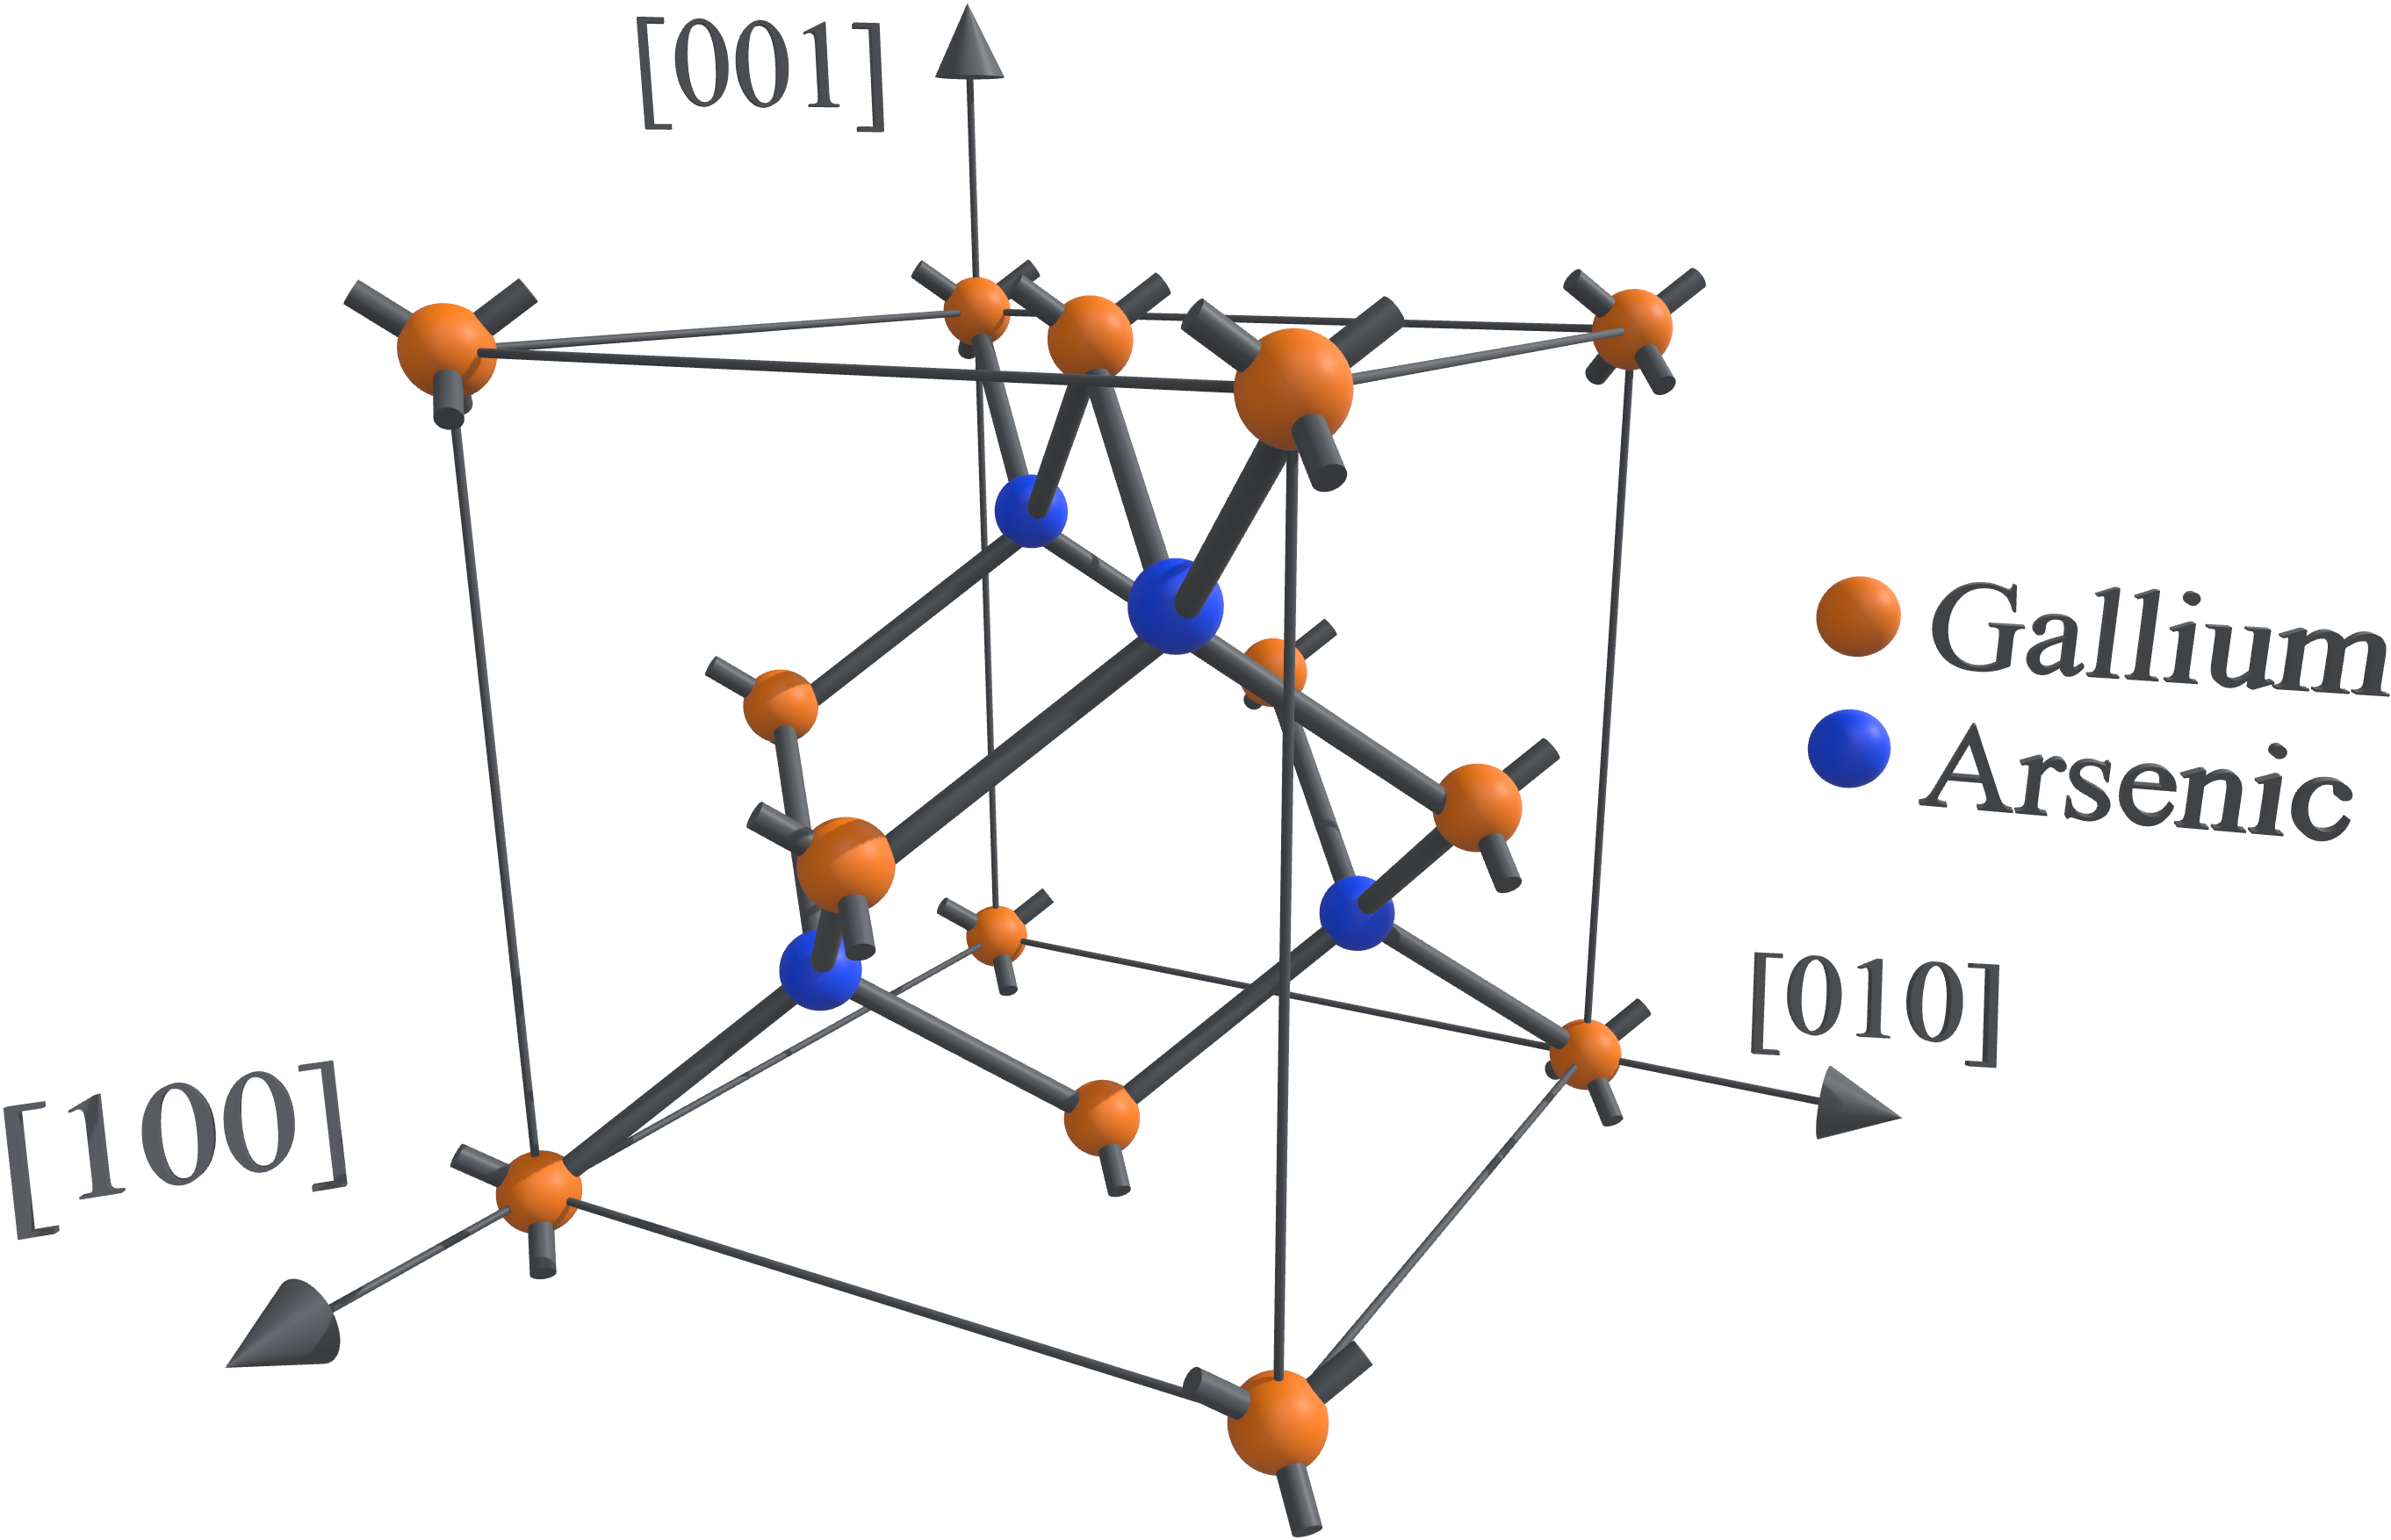
\includegraphics[width=\textwidth]{figs/ALGAAS/gaas_unit_cell_mi.PNG}
\caption{The unit cell of gallium arsenide (GaAs) with associated miller indices as coordinate axes}
\label{fig:gaas_uc}
\end{figure}

\textcolor{red}{Mention the difference in lattice cell constant between $\gaas$ and $\algaas$?}


\subsection{Induced anisotropy in zincblende crystals}
Zincblende structures, like the crystalline materials in question can exhibit birefringent properties when under the influence of two factors: stress in the material, and present within DC electric fields. These two properties of crystalline materials are known as the photoelastic and electro-optic effects respectively.

\subsubsection{The (linear) electro-optic (Pockel's) effect}

For non-centrosymmetric crystalline media there exists a non-zero rank 2, $6 \times 3$ tensor ($r_{ij}$) connecting a low-frequency \footnote{"low frequency" meaning orders of magnitude smaller than an optical field it effects} electric field $\vec{E}(f) = [E_x(f), E_y(f), E_z(f)]$ directly to the \hyperref[sec:indicatrix]{indicatrix} ~\cite{yariv,nye}:
\begin{equation}
  \left[ {\begin{array}{c}
   \big( \frac{1}{\Delta n ^2 } \big)_1 \\
   \big( \frac{1}{\Delta n ^2 } \big)_2 \\
   \big( \frac{1}{\Delta n ^2 } \big)_3 \\
   \big( \frac{1}{\Delta n ^2 } \big)_4 \\
   \big( \frac{1}{\Delta n ^2 } \big)_5 \\
   \big( \frac{1}{\Delta n ^2 } \big)_6 \\
  \end{array} } \right]
  =
%
 \left[ {\begin{array}{ccc}
   r_{11} & r_{12} & r_{13}\\
   r_{21} & r_{22} & r_{23}\\
   r_{31} & r_{32} & r_{33}\\
   r_{41} & r_{42} & r_{43}\\
   r_{51} & r_{52} & r_{53}\\
   r_{61} & r_{62} & r_{63}\\
  \end{array}} \right]
 %
 \left[{\begin{array}{c}
   E_x (f)\\
   E_y (f)\\
   E_z (f)\\
 \end{array}} \right]
\end{equation}

\noindent The $i$ index runs over the terms in the indicatix equation:
\begin{equation}
\bigg(\frac{1}{\Delta n_x^2} \bigg) x^2\ + \bigg(\frac{1}{\Delta n_y^2} \bigg) y^2 + \bigg(\frac{1}{\Delta n_z^2} \bigg) z^2 + 2 \bigg(\frac{1}{\Delta n_{xz}} \bigg)xz + 2 \bigg(\frac{1}{\Delta n_{yz}} \bigg)yz + 2 \bigg(\frac{1}{\Delta n_{xy}} \bigg)xy = 1
\end{equation}

\noindent \textcolor{red}{Detail on some prior knowledge of $f \leq f_\mathrm{max}$? (Pockels cell specs?)}


\subsubsection{$r_{ij}$ for zincblende crystals ($r_{\bar{4}3m, ij}$)}

The form of the electro-optic tensor for zincblende crystals (including $\gaas$ and $\algaas$) reduces such that $r_{ij} = r_{41} = r_{52} = r_{62} \neq 0$ with all other terms being zero:

\begin{equation}
r_{\bar{4}3m,ij} =
 \left[ {\begin{array}{ccc}
  0 & 0 & 0\\
  0 & 0 & 0\\
  0 & 0 & 0\\
  r_{41} & 0 & 0\\
  0 & r_{52} & 0\\
  0 & 0 & r_{63}\\
 \end{array}} \right]
\end{equation}

\noindent Where also $r_{41} = r_{52} = r_{63}$

\subsubsection{New principal (electro-optic) dielectric axis for zincblende structures}

In general the principle dielectric axes of the new ellipsoid do \textbf{not} coincide with the axes of the ellipsoid of the unperturbed crystal. The form of the index ellipsoid for a zincblende crystalline material accounting for the electro-optic tensor and some generalized DC electric field $\vec{E}$ expressed in terms of the crystallographic axes is given by:
\begin{equation}\label{eq:zindicatrix}
\bigg(\frac{1}{n_o^2} \bigg) x^2\ + \bigg(\frac{1}{n_o^2} \bigg) y^2 + \bigg(\frac{1}{n_o^2} \bigg) z^2  + 2r_{41} E_{[100]} yz + 2r_{41} E_{[010]} xz + 2r_{41}E_{[001]} xy= 1
\end{equation}

\noindent Where we have set $n_x = n_y = n_z = n_o$ for zincblende structures.

\noindent The two principal axes are given by the eigenvectors of the the matrix given from the equation above:

\begin{equation}
 \left[ {\begin{array}{ccc}
   \big( \frac{1}{n_o ^2} \big)& r_{41}E_{[001]} & r_{41} E_{[010]}\\
   r_{41}E_{[001]} & \big( \frac{1}{n_o ^2} \big) &  E_{[100]}\\
   r_{41} E_{[010]} & r_{41} E_{[100]} & \big( \frac{1}{n_o ^2} \big)\\
  \end{array}} \right]
\end{equation}

\subsubsection{The photoelastic effect?}

When a general strains $S_{kl}(r) = \frac{1}{2} \bigg[ \frac{\partial u_k (r)}{\partial x_i} + \frac{\partial u_i (r)}{\partial x_k} \bigg]$ are applied to a material, the photoelastic tensor $p_{idkl}$ relates to the indicatrix by the following relation:

\begin{equation}
 \bigg( \frac{1}{\Delta n^2} \bigg)_{id} = p_{idkl} S_{kl}
\end{equation}

\textcolor{red}{Supplementary comment to the measured birefringence from the mentioned intrinsic strain of the high and low index layers}

\subsubsection{The generalized indicatrix}

\subsubsection{New principal dielectric axes for zincblende structures (zinblende photoelastic tensor, zincblende electro-optic tensor)}

\subsection{Electro-optic modulation}\label{sec:EOM}
A common application of this effect is phase modulation onto a optical carrier field. Electro-optic modulators or Pockel cells accomplish this by sandwiching two capacitor plates around crystal with a single electrical input port designed to take in a frequency ($\Omega$) within a specified modulation bandwidth. When the field amplitude across the crystal is driven by a voltage controlled oscillation, we exiperience a change in the electro-optic tensor The voltage amplitude of the signal input is proportional to the strength of the phase modulation on the optical carrier field of frequency ($\omega$) and is commonly quantified in terms of a modulation index ($\beta$).

\textcolor{red}{FIGURE: Longitudinal and Transverse EOMs}

\textcolor{red}{Consider specific crystal that gives us our $\beta \mathrm{sin}(\Omega t)$}


Consider orientation

\begin{equation}
E_\mathrm{inp} = E_o e^{i \omega t + \beta \mathrm{sin}( \Omega t)}
\end{equation}

If the modulation depth is set such that $\beta < 1$ then the input field may be approximated in terms of the first two Bessel functions $J_0$, $J_1$:

\begin{equation} \label{eq:EOM_trans_field}
E_\mathrm{inp} \approx E_0 [J_0(\beta)e^{i \omega t} + J_1(\beta)e^{i (\omega + \Omega) t} - J_1(\beta)e^{i(\omega -\Omega)t}]
\end{equation}

\textcolor{red}{This construction resembles that of the electrostatic optical mount used to drive a longitudinal electric field}

\subsection{Optical anisotropy of a HR $\gaas$ / $\algaas$ stack}
Our interests primarily lie with the study of birefringent properties of a candidate highly reflective $\gaas$/$\algaas$ mirrorstack. This section is intended to provide a comprehensive review by: 1) making considerations of crystal coordinates when asserting an optical axis on a highly reflective crystalline stack manufactured by Thorlabs, 2) citing coating parameters and observed intrinsic birefringence from the highly reflective coating stack in question, 3) analyzing differential linear electro-optic effect on the phase of a reflected beam, and 4) estimating the the differential phase noise in LIGO based on calibrated electric field measurements.
%\subsubsection{Growth orientation (Miller indices) with respect to substrate surface}
%\begin{itemize}
%\item Mirror surface is the [100] plane.
%\item Within the [100] plane the AlGaAs coating is grown with a flat indicator that draws a line within the [0-11] plane where the bisected line points towards the sample center.
%\end{itemize}

\subsubsection{Miller indices for highly reflective coatings $\gaas$/$\algaas$ coatings}
\begin{figure}[H]
\begin{center}
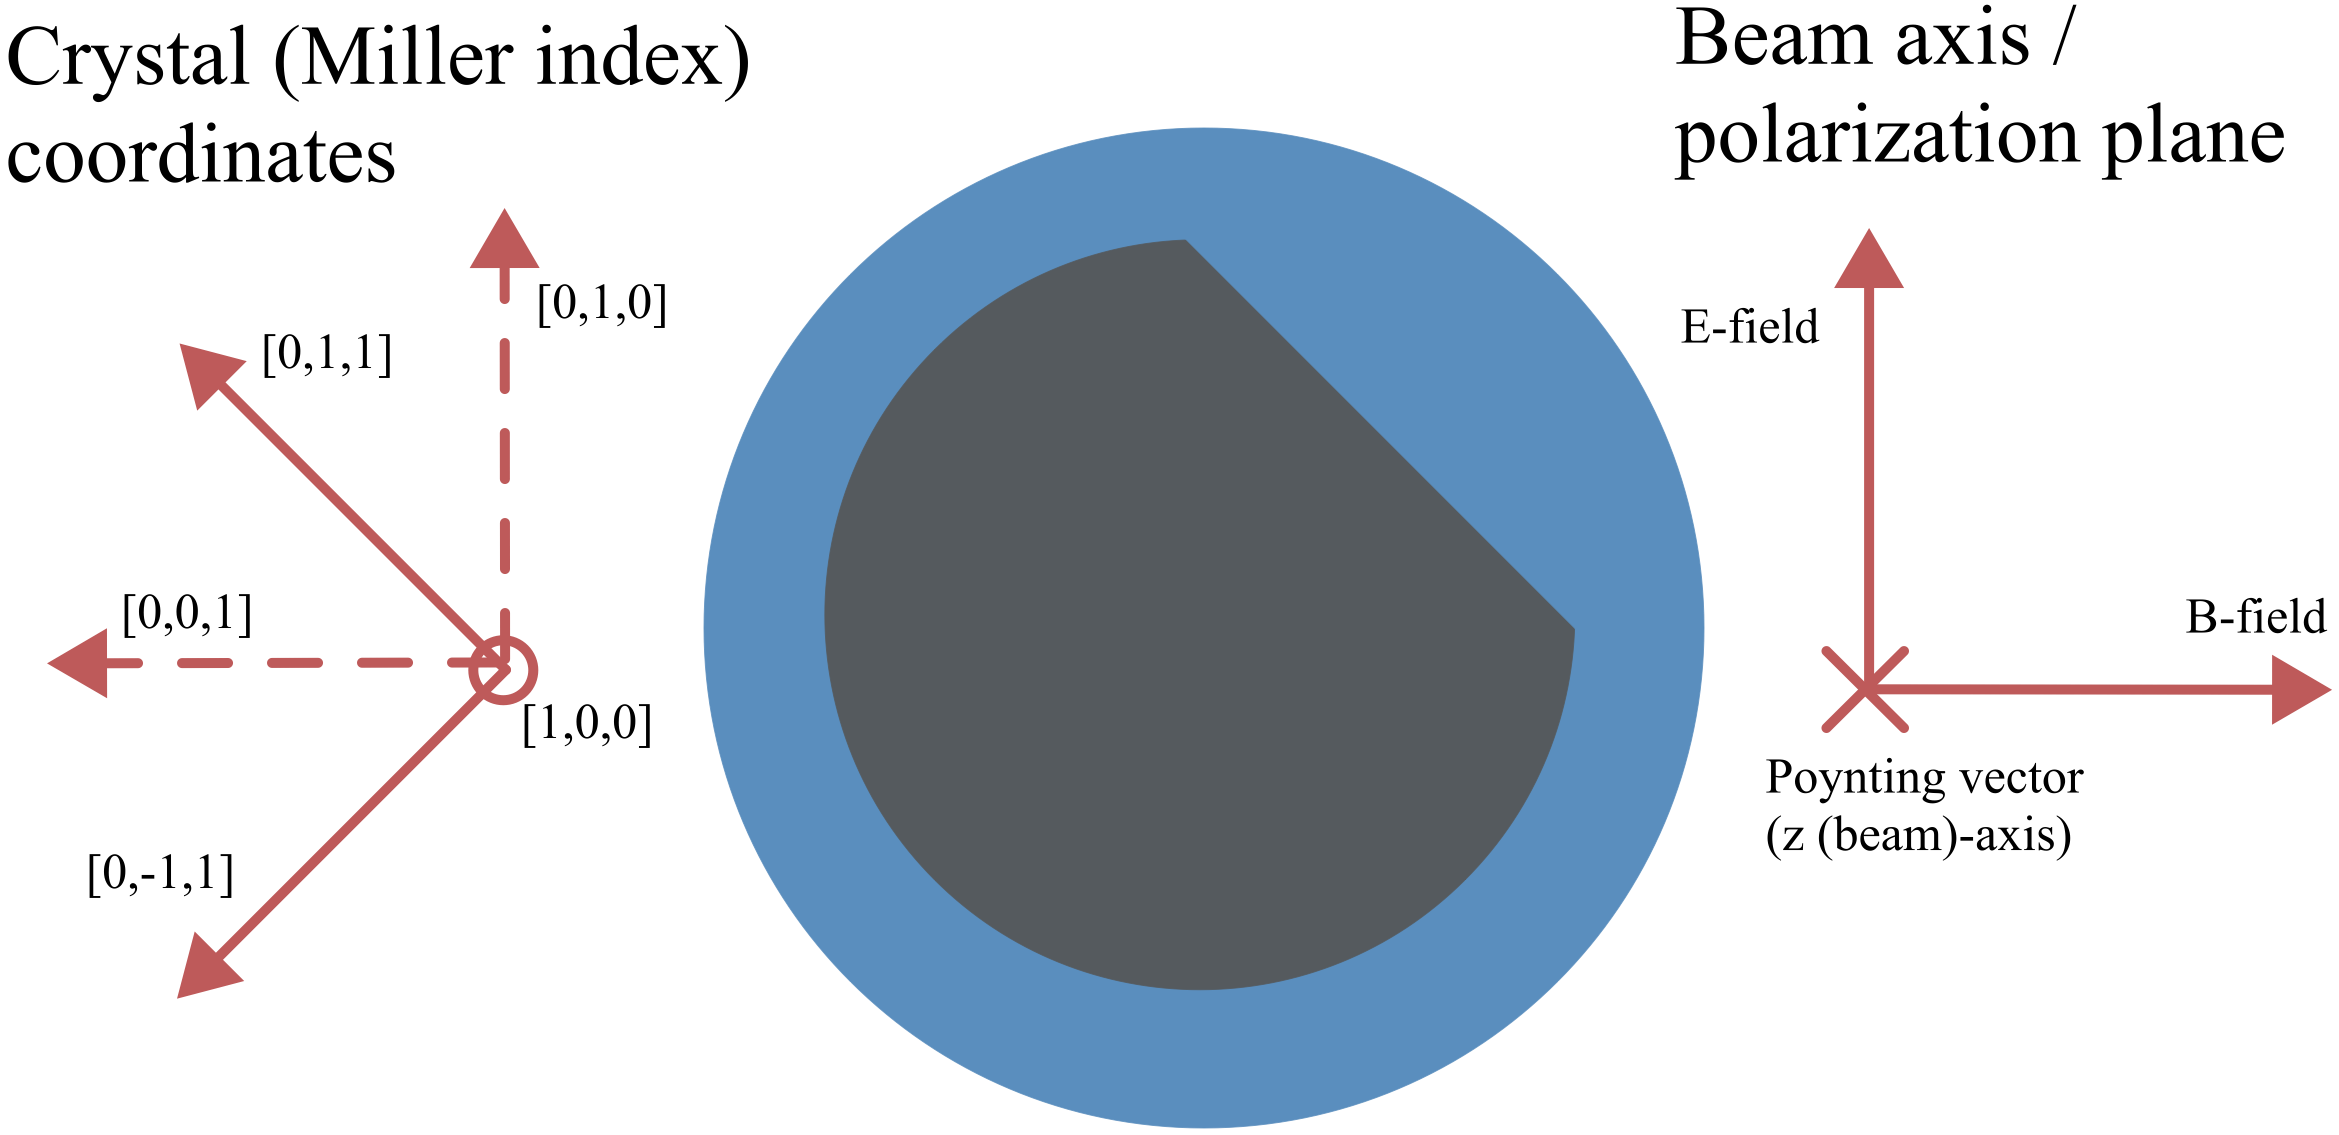
\includegraphics[width=\textwidth]{figs/ALGAAS/algaas_sample_diagram.png}
\end{center}
\caption{\textcolor{red}{PENDING UPDATES} Figure of the beam propogation axis with respect to the AlGaAs/GaAs crystal axes (not final version). Within the [100] plane the AlGaAs coating is grown with a flat indicator that draws a line within the [0-11] plane where the bisecting vector of the plane normal points towards the sample center. The axis formed by the [100] is parallel with the beam axis (z-axis). The polarizations of incident and reflected beam oscillate along vectors within the plane formed by the normal of that axis.}
\label{fig:algaas_coords}
\end{figure}

Up until this point we have discussed three different coordinate axes: the crystal axis (indicated by Miller index plane normals), the principal dielectric axis (coordinates based in diagonalization of the indicatrix), and an optical axis (when considering a desired (laser) light propogation). We assert the beam axis \cite{fig:algaas_coords} with linearly p-polarized light.
\begin{figure}[H]
\begin{center}
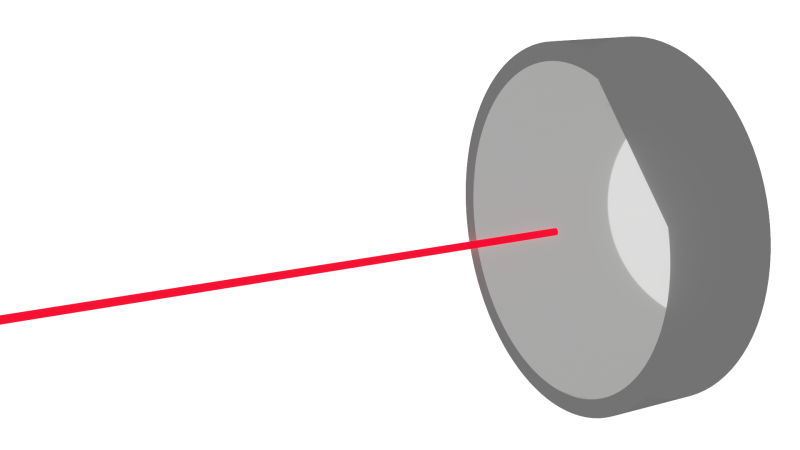
\includegraphics[width=.45\textwidth]{figs/ALGAAS/laser_mirror_test2.png}
\end{center}
\caption{Laser AlGaAs mirror figure test}
\label{fig:algaas_mirror}
\end{figure}
\subsubsection{Electro-optic coupling to the reflected phase of a HR mirror coating}
With our coordinate considerations and established beam axis, it is now worth considering the influence of an isotropic white noise field ($E_n = [E_{nx},E_{ny},E_{nz}]$):

\begin{equation}
 \left[ {\begin{array}{ccc}
   \big( \frac{1}{n_o ^2} \big)& r_{41}E_{ny} & r_{41} E_{nx}\\
   r_{41}E_{ny} & \big( \frac{1}{n_o ^2} \big) & r_{41} E_{nz}\\
   r_{41} E_{nx} & r_{41} E_{ny} & \big( \frac{1}{n_o ^2} \big)\\
  \end{array}} \right]
\end{equation}

Assuming $E_n$ is small, the indicatrix change of $E_{nx}$ and $E_{ny}$ relative to $E_{nz}$ (as seen by the beam polarization) will be small ($r_{41}E_{n(x/y)} \ll r_{41}E_{nz}$). After diagonalizing with relevant terms \footnote{Note that the form of the tensor is still in the crystal coordinates but the $E_n$ terms are placed in the tensor such that their directions align with beam axis coordinates.} in the tensor, we are left with the following eigenindices:

\begin{equation}
\begin{aligned}
n_x' & = n_o - r_{41}E_{nz} \\
n_y' & = n_o + r_{41}E_{nz}
\end{aligned}
\end{equation}

%\textcolor{red}{How the modulation of the phase of the carrier field is dependent on the orientation of its wave vector with respect to the crystal structure, the modulating electric field direction and strength, (other items to discuss in terms of introducing the effect)}
For GaAs @ $10.6\mu$ $r_{41} = 1.6 \times 10^{-12}$ [m/V]
\\
Adachi estimate for $\mathrm{Al_{x}Ga_{1-x}As}$?
\\
\textcolor{red}{Relevant eigenpolarizations, non-optical field $E_y = E_z = 0$?}
\\
\textcolor{red}{Figure: Transformed indicatrix (Before and after $E_x$)}
\\
\textcolor{red}{Figure: Ellipse cross section. New eigenpolarizations and corresponding indices and their influence on incident field (Marty's result)}
\\
Assuming we are operating in a coordinate system suggested in \hyperref[fig:algaas_coords]{Figure ?}. Given this configuration, which plane is impacted by some $E_\mathrm{noise}$? Revisiting the \hyperref[eq:zindicatrix]{indicatrix}. We can see that for even non-zero z and y components that the only coupling to the input beam polarization is the index along the cross coupled zy axis through $E_z$ is that of the $E_x$ term. This gives us the ability to easily diagonalize the indicatrix tensor by setting the non-relevant field terms to zero.
Fejer and Bonilla take an analytical approximation approach when finding the impact of the electric field to the change in phase of the light through a crystalline anisotropic thin film ($\lambda/4$) stack \cite{bonilla_fejer}.

\begin{equation}
\hat{\phi}' = \frac{\pi n_1 z}{1-z^2}(z^{2N} -1) \frac{z^{2N} \frac{(n_f)^2}{n_2 n_3}(n_2 \kappa_{\gamma 2} + n_3\kappa_{\gamma 3}) - (n_2 \kappa_{\gamma 3} + n_3\kappa_{\gamma 3})}{(n_1)^2 -(n_f)^2 z^{4N}}
\end{equation}

with $z = \frac{n_2}{n_3}$
and
$
\kappa_{\gamma j} = \frac{d}{d \gamma} \mathrm{log}(n_j h_j)|_{\gamma =\gamma_{O}} \bigg(\frac{\hat{n}_j'}{\hat{n}_j} +\frac{\hat{h}_j'}{\hat{h}_j} \bigg)
$

With $\kappa$ being a scalar parameter.

\satoshi{Adding a schematic would be helpful.}

\textcolor{red}{Figure is in the works}

\subsubsection{Numerically friendly estimate}

In the appendix of \cite{ballmer2015} Ballmer constructs a coating layer transfer function for a given coating layer k with index $n_k$, and thickness $d_k$, defining right and left propogating modes $\Psi^{R,L}$ repsectively:

\begin{equation}
  \left[ {\begin{array}{c}
   \Psi^\mathrm{R} \\
   \Psi^\mathrm{L} \\
  \end{array} } \right]_{k+1}
  =
%
Q_k D_k
%
 \left[{\begin{array}{c}
   \Psi^\mathrm{R} \\
   \Psi^\mathrm{L} \\
 \end{array}} \right]
\end{equation}

\noindent $D_k$ applies the phase ($\phi_k = 4\pi n_k d_k /\lambda_0$) from a given coating layer, and $Q_k$ applies the transfer function between high-low/low-high index layers transition:

\begin{equation}
Q_k = \frac{1}{2n_{k+1}}
\left[ {\begin{array}{cc}
  n_{k+1} + n_k & n_{k+1} - n_k\\
 n_{k+1} - n_k & n_{k+1} + n_k\\
\end{array} } \right]
\end{equation}

\begin{equation}
D_k =
\left[ {\begin{array}{cc}
  e^{-i \phi_k / 2}& 0\\
 0 & e^{i \phi_k / 2}\\
\end{array} } \right]
\end{equation}
Defining a HR coating stack, the total transfer matrix from vaccum $Q_0$ to the $N$th coating layer is:
\begin{equation}
M = Q_N D_N ...Q_kD_k...Q_1D_1Q_0
\end{equation}
The impact of a differential electric noise field ($E$) on $M$ due to the electro-optic effect on the kth layer, we use the chain rule:


The coating to be studied consists 36 $\lambda$/4  thick layers of $\gaas$ interspersed with 35 layers of $\lambda$/4 thick $\algaas$.   $\gaas$ forms the top and bottom layer to prevent oxygen absorption from the AlGaAs layer. The $\gaas$ layers have an index of $n_{\gaas} = 3.480$ and a thickness of $\Delta d_{\gaas} = 76.43$ nm while the low index $\algaas$ layers are $n_{\algaas} = 2.977$ with thickness $\Delta d_{\algaas} = 89.35$ nm. With the cosntructed matrices, we apply these parameters and compute a differential phase of:

%High Index:  GaAs, n=3.480, layer thickness is 76.43 nm
%Low Index:  $ \mathrm{Al}_{0.92} \mathrm{Ga}_{0.08} \mathrm{As} $, n=2.977, layer thickness is 89.35 nm
%\textcolor{red}{Info from Steve. Written source?}


\subsection{Measured birefringence from HR $\gaas$/$\algaas$ mirrors}
There seems to be different accounts of a measured birefringence from HR $\gaas$ / $\algaas$ (\href{https://dcc.ligo.org/DocDB/0181/G2200386/001/G2200386.pdf}{Satoshi}, \href{https://nodus.ligo.caltech.edu:8081/CTN/1474}{CTN}, \href{https://dcc.ligo.org/DocDB/0181/G2200559/001/G2200559-v1%20-%20polarization.pdf}{Aidan})
\\
\textcolor{red}{Is the measured birefringence static? (Layer bonding method might introduce something?)}
\\
\textcolor{red}{Does it change from different mounting methods? (Photoelastic) (order of magnitude estimate)}
%\\
%\textcolor{red}{Electro-optic ruled out based on field measurements and relative coupling factor.}
\\
\textcolor{red}{Measurement precision of the coating birefringence? Cavity length, Polarization drifts, etc.}
\\
The measured birefringence is estimated to be caused by an intrinsic strain between the epitaxial layers of $\gaas$/$\algaas$. \cite{Cole:2013}
\\
\textcolor{red}{Marty's document about Birefringence in Crystalline mirror coatings V.8}

\section{Projected DARM coupling}
To estimate how much DARM coupling can occur, we use use a measured field spectra acquired from installed electric field meters located within LIGO Hanford Observatory EX and EY vacuum chambers. Taking the upper and the lower EFM measurements in $.3\; [\mathrm{V}/\mathrm{m}/\sqrt{\mathrm{Hz}]}$ @ 60 Hz and $4\times10^{-3}\; [\mathrm{V}/\mathrm{m}/\sqrt{\mathrm{Hz}]}$ @ 4kHz ~\cite{efm_log}.
\satoshi{I don't think these values are calibrated. According to Martynov et al. 2016, the fluctuations in the electric filed is $\sim10^{-5}\,\mathrm{[(V/m)/\sqrt{Hz}]}$.}
This along with computed estimate above allows us to create an upper limit for what this noise might be assuming incoherent fields between the end stations and a flat frequency response within LIGO's bandwidth.

\section{Experiment}
The motivation behind this work was generating a calibrated estimate of the pockels effect from a $\gaas$/$\algaas$ mirror sample from Thorlabs' crystalline mirror coatings. As seen in the prior section, the size of the imparted phase noise, for currently existing gravitational wave detector configurations, is estimated to be small but notable. Investigation through measurement of said effect requires detection methods with sufficient sensitivity for the differential phase noise imparted by the effect. Lock-in detection via a Pound-Drever-Hall servo to maintain resonance of a 1064nm carrier field to a Fabry-Perot cavity, with the aforementioned crystalline coated cavity end mirror installed in a custom longitudinal pockels cell mirror mount around was tried. Details and specifications of the detection scheme are discussed along with relevant measurements and results.

\subsection{Lock-In detection scheme}
\begin{figure}[H]
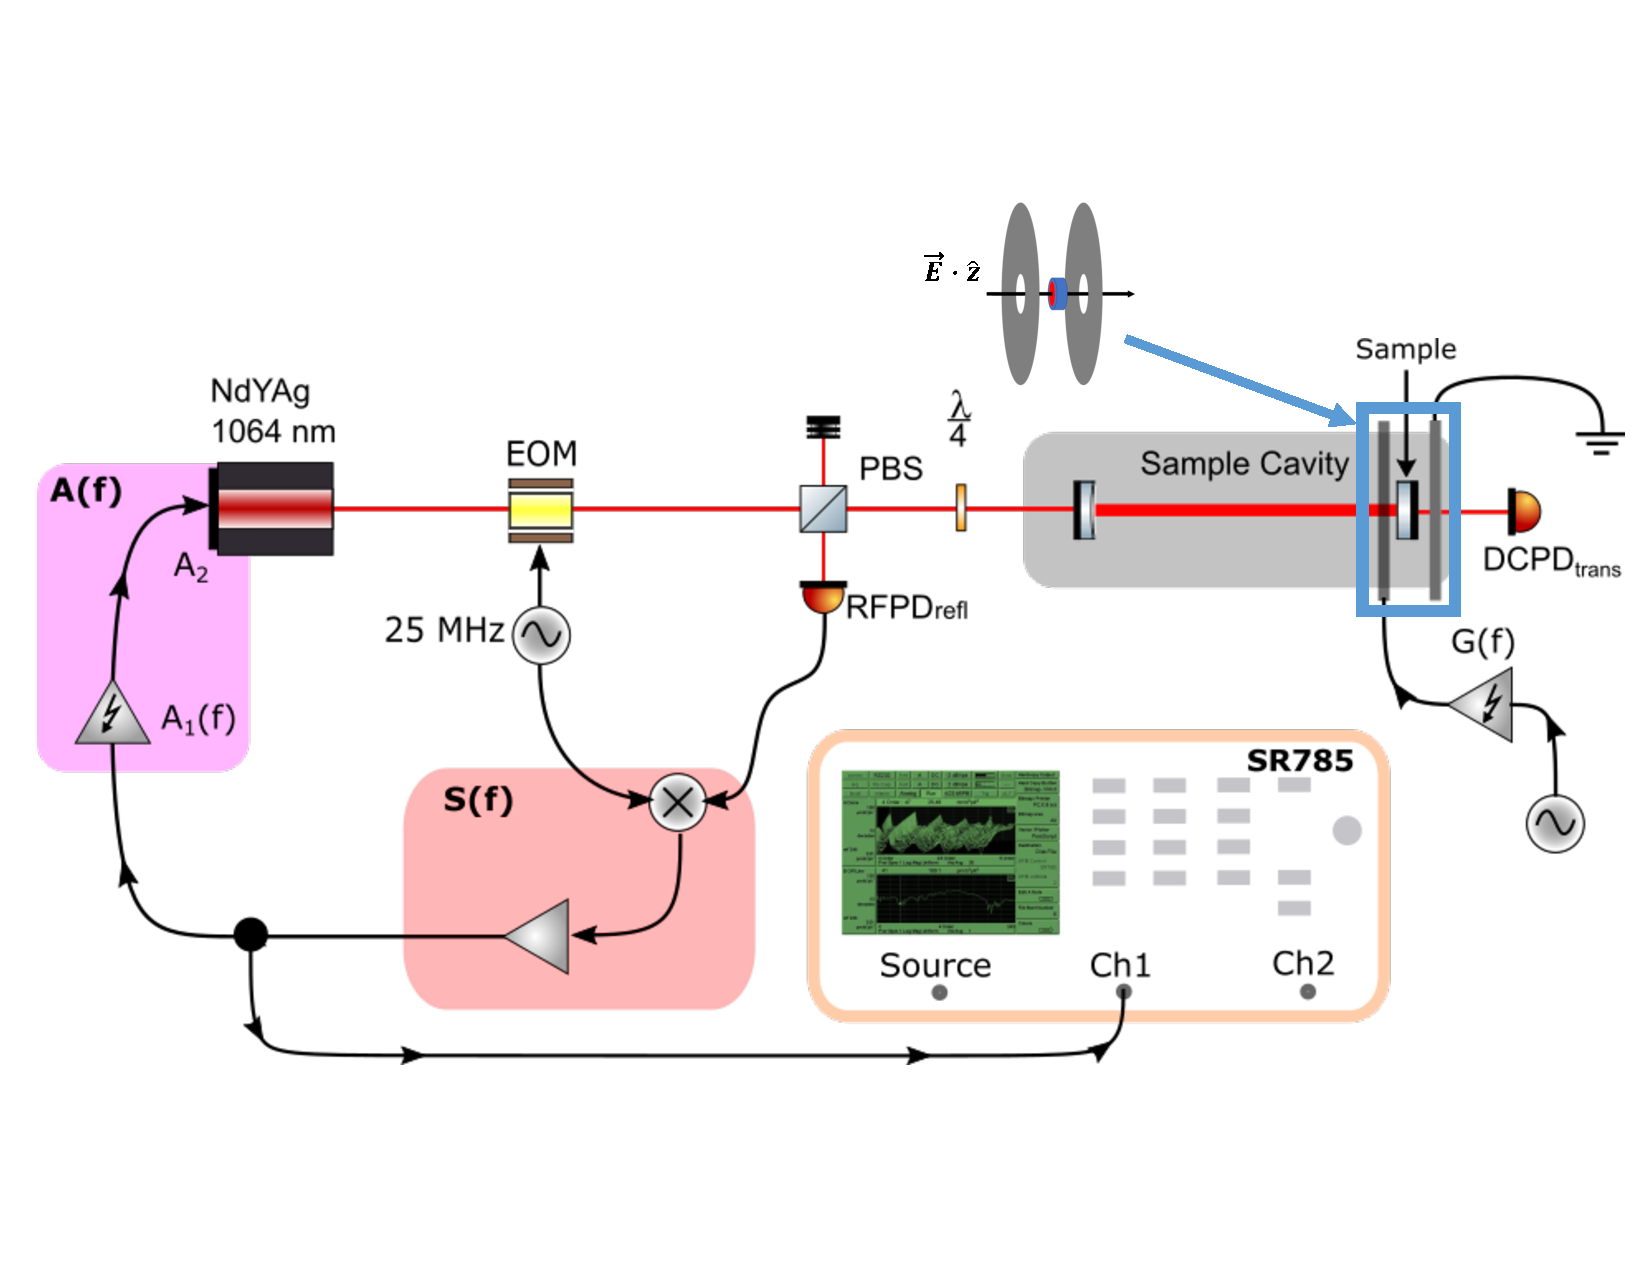
\includegraphics[width=\textwidth]{figs/ALGAAS/algaas_pockels_effect_measurement_schematic.pdf}
\caption{A simplified and modular schematic of the PDH servo used along with an electrostatic drive mount design comprised of a disk capacitor sandwiching the HR AlGaAs sample, a high voltage amplifier, and a signal / network analyzer.}
\label{fig:simplified_experiment_schema}
\end{figure}
The size of the effect calls for a detection scheme allowing measurement of signals with low SNR, hence the choice for lock-in. Measurability of the electro-optic effect is also contingent upon two initial design criteria: the sensitivity of the optical plant to be implemented in the PDH servo, and the maximum achievable electric field strength along the beam axis ($|E_z|_\mathrm{max}$).

\subsubsection{PDH servo}\label{subsubsec:pdh}
The Pound-Drever-Hall technique, originally imagined for laser frequency stabilization to an ultra-stable length reference, allows the tracking of the linear phase response of an input carrier field through cavity resonance. The servo fully realizes the ability of an optical cavity to act as a length / frequency discriminator. The alternative cavity offset lock provides a linear response in intensity, which is adequate for some applications but with reduced sensitivity due to the required power reduction by operating off resonance.
\begin{figure}[H]
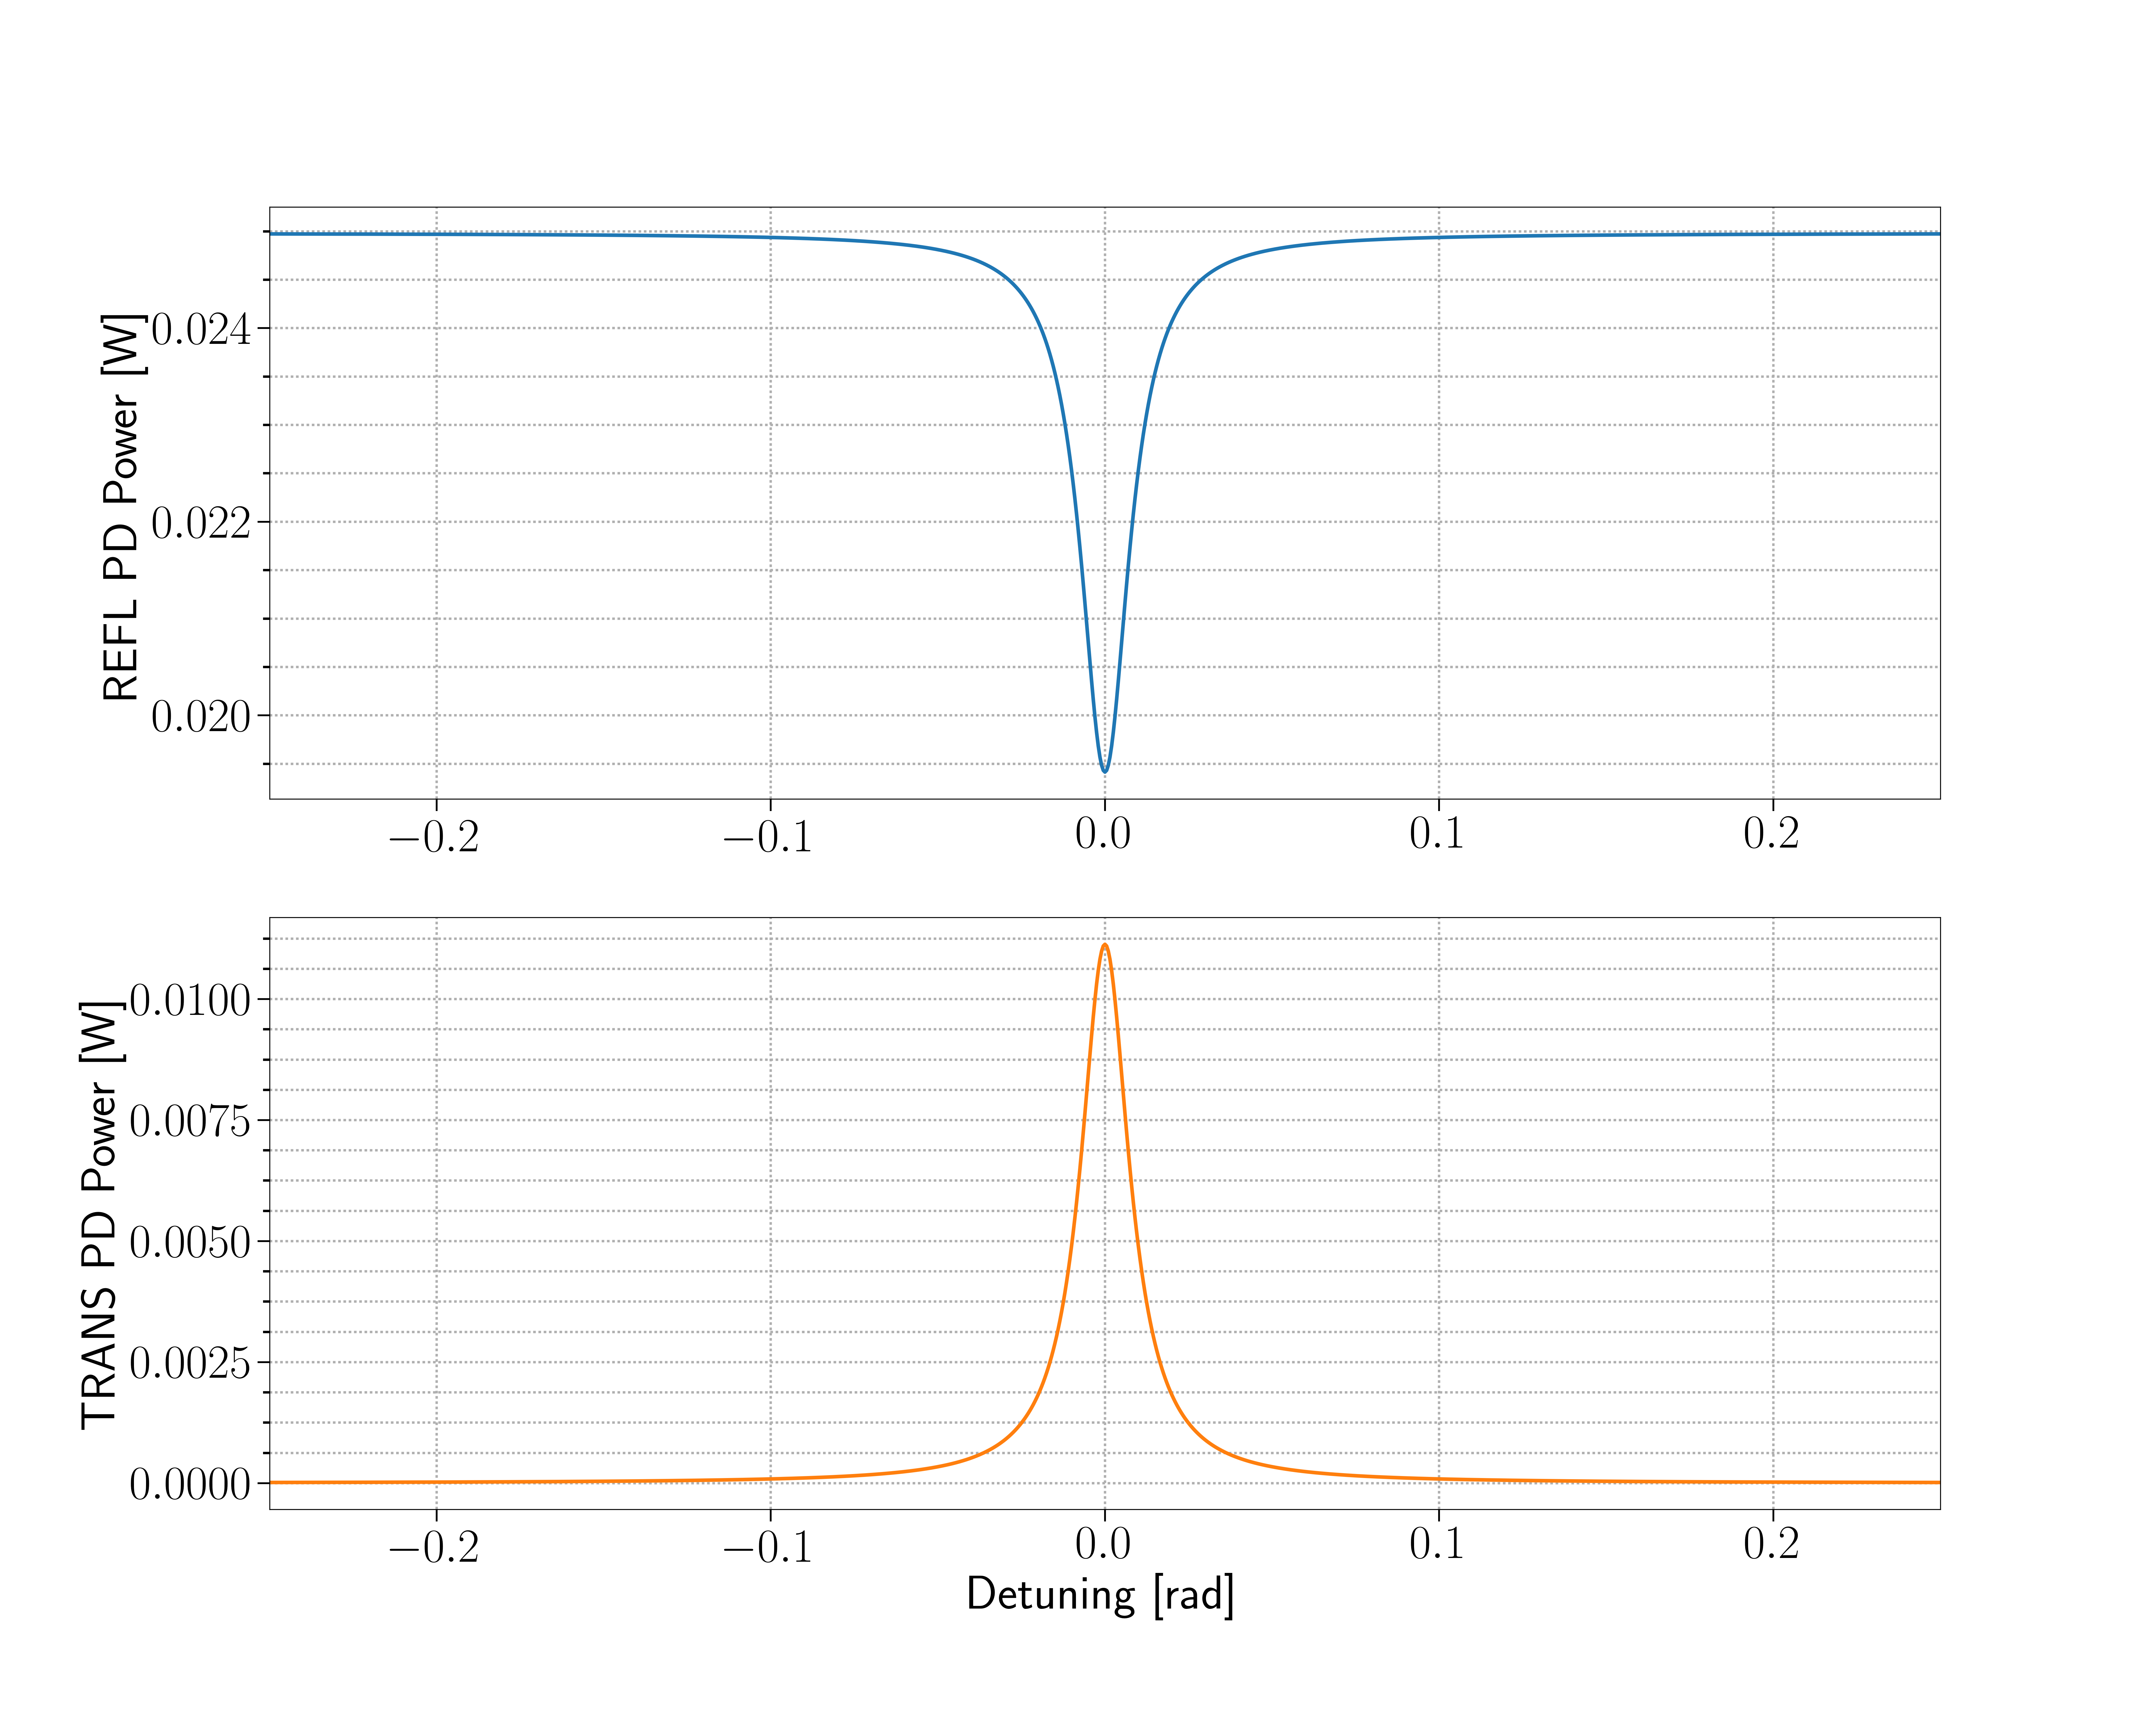
\includegraphics[width=\textwidth]{figs/ALGAAS/DC_power_cav_resonance.png}
\caption{Reflected and transmitted power around resonance.
\textcolor{red}{Phase as dotted line?}}
\label{fig:cav_length_response_DCpow}
\end{figure}
Th phase measurement is achieved through an optical heterodyne; the co-propogation of a separate (but phase-locked) optical field with a known frequency separation to the carrier reflected from the cavity input. To accomplish this, the PDH servo offers a way to avoid complicated phase-locked two laser configurations, by imposing a phase modulation on the carrier field via an electro-optic modulator (aka Pockels cell) mentioned in section \ref{sec:EOM}. With a high enough modulation frequency, phase modulation onto the carrier field is mathematically and physically equivalent to imposing separate optical fields (sidebands) which in most cases do not resonate in the optical cavity of interest. Setting a photodiode of area ($A_\mathrm{PD}$) in reflection of the cavity reflection coefficient of $r_\mathrm{cav}(\omega,L)$, we measure the reflected power of the input field given by \ref{eq:EOM_trans_field}:

\begin{equation}
 \begin{alignedat}{3}
    &P_\mathrm{refl} && \approx \frac{|E_\mathrm{refl}|^2}{A_\mathrm{PD}} && \\
    & &&\approx \frac{E_0^2}{A_\mathrm{PD}} && \bigg\{J_0^2 |r_\mathrm{cav}(\omega,L)|^2 + J_1^2(\beta)|r_\mathrm{cav}(\omega+\Omega,L)|^2 - J_1^2(\beta)|r_\mathrm{cav}(\omega-\Omega,L)|^2 +  \\
    & && && J_0J_1(\beta)\big[r_\mathrm{cav}\omega,L) r_\mathrm{cav}^*(\omega+\Omega,L)\big] - J_ 0J_1(\beta)\big[r_\mathrm{cav}(\omega,L)r_\mathrm{cav}^*(\omega-\Omega,L)\big]\bigg\}
  \end{alignedat}
\end{equation}

The two trailing terms in the above equation for $P_\mathrm{refl}$ generate a beat frequency term between the carrier and lower and upper sidebands. The magnitude and sign of these beat terms directly relate to the phase of the reflected carrier field and can be measured and transformed to the error signal seen in \ref{fig:pdh_error} using resonant electronics (tuned to a chosen sideband frequency) for amplification and a mixer for demodulation.

\begin{figure}[H]
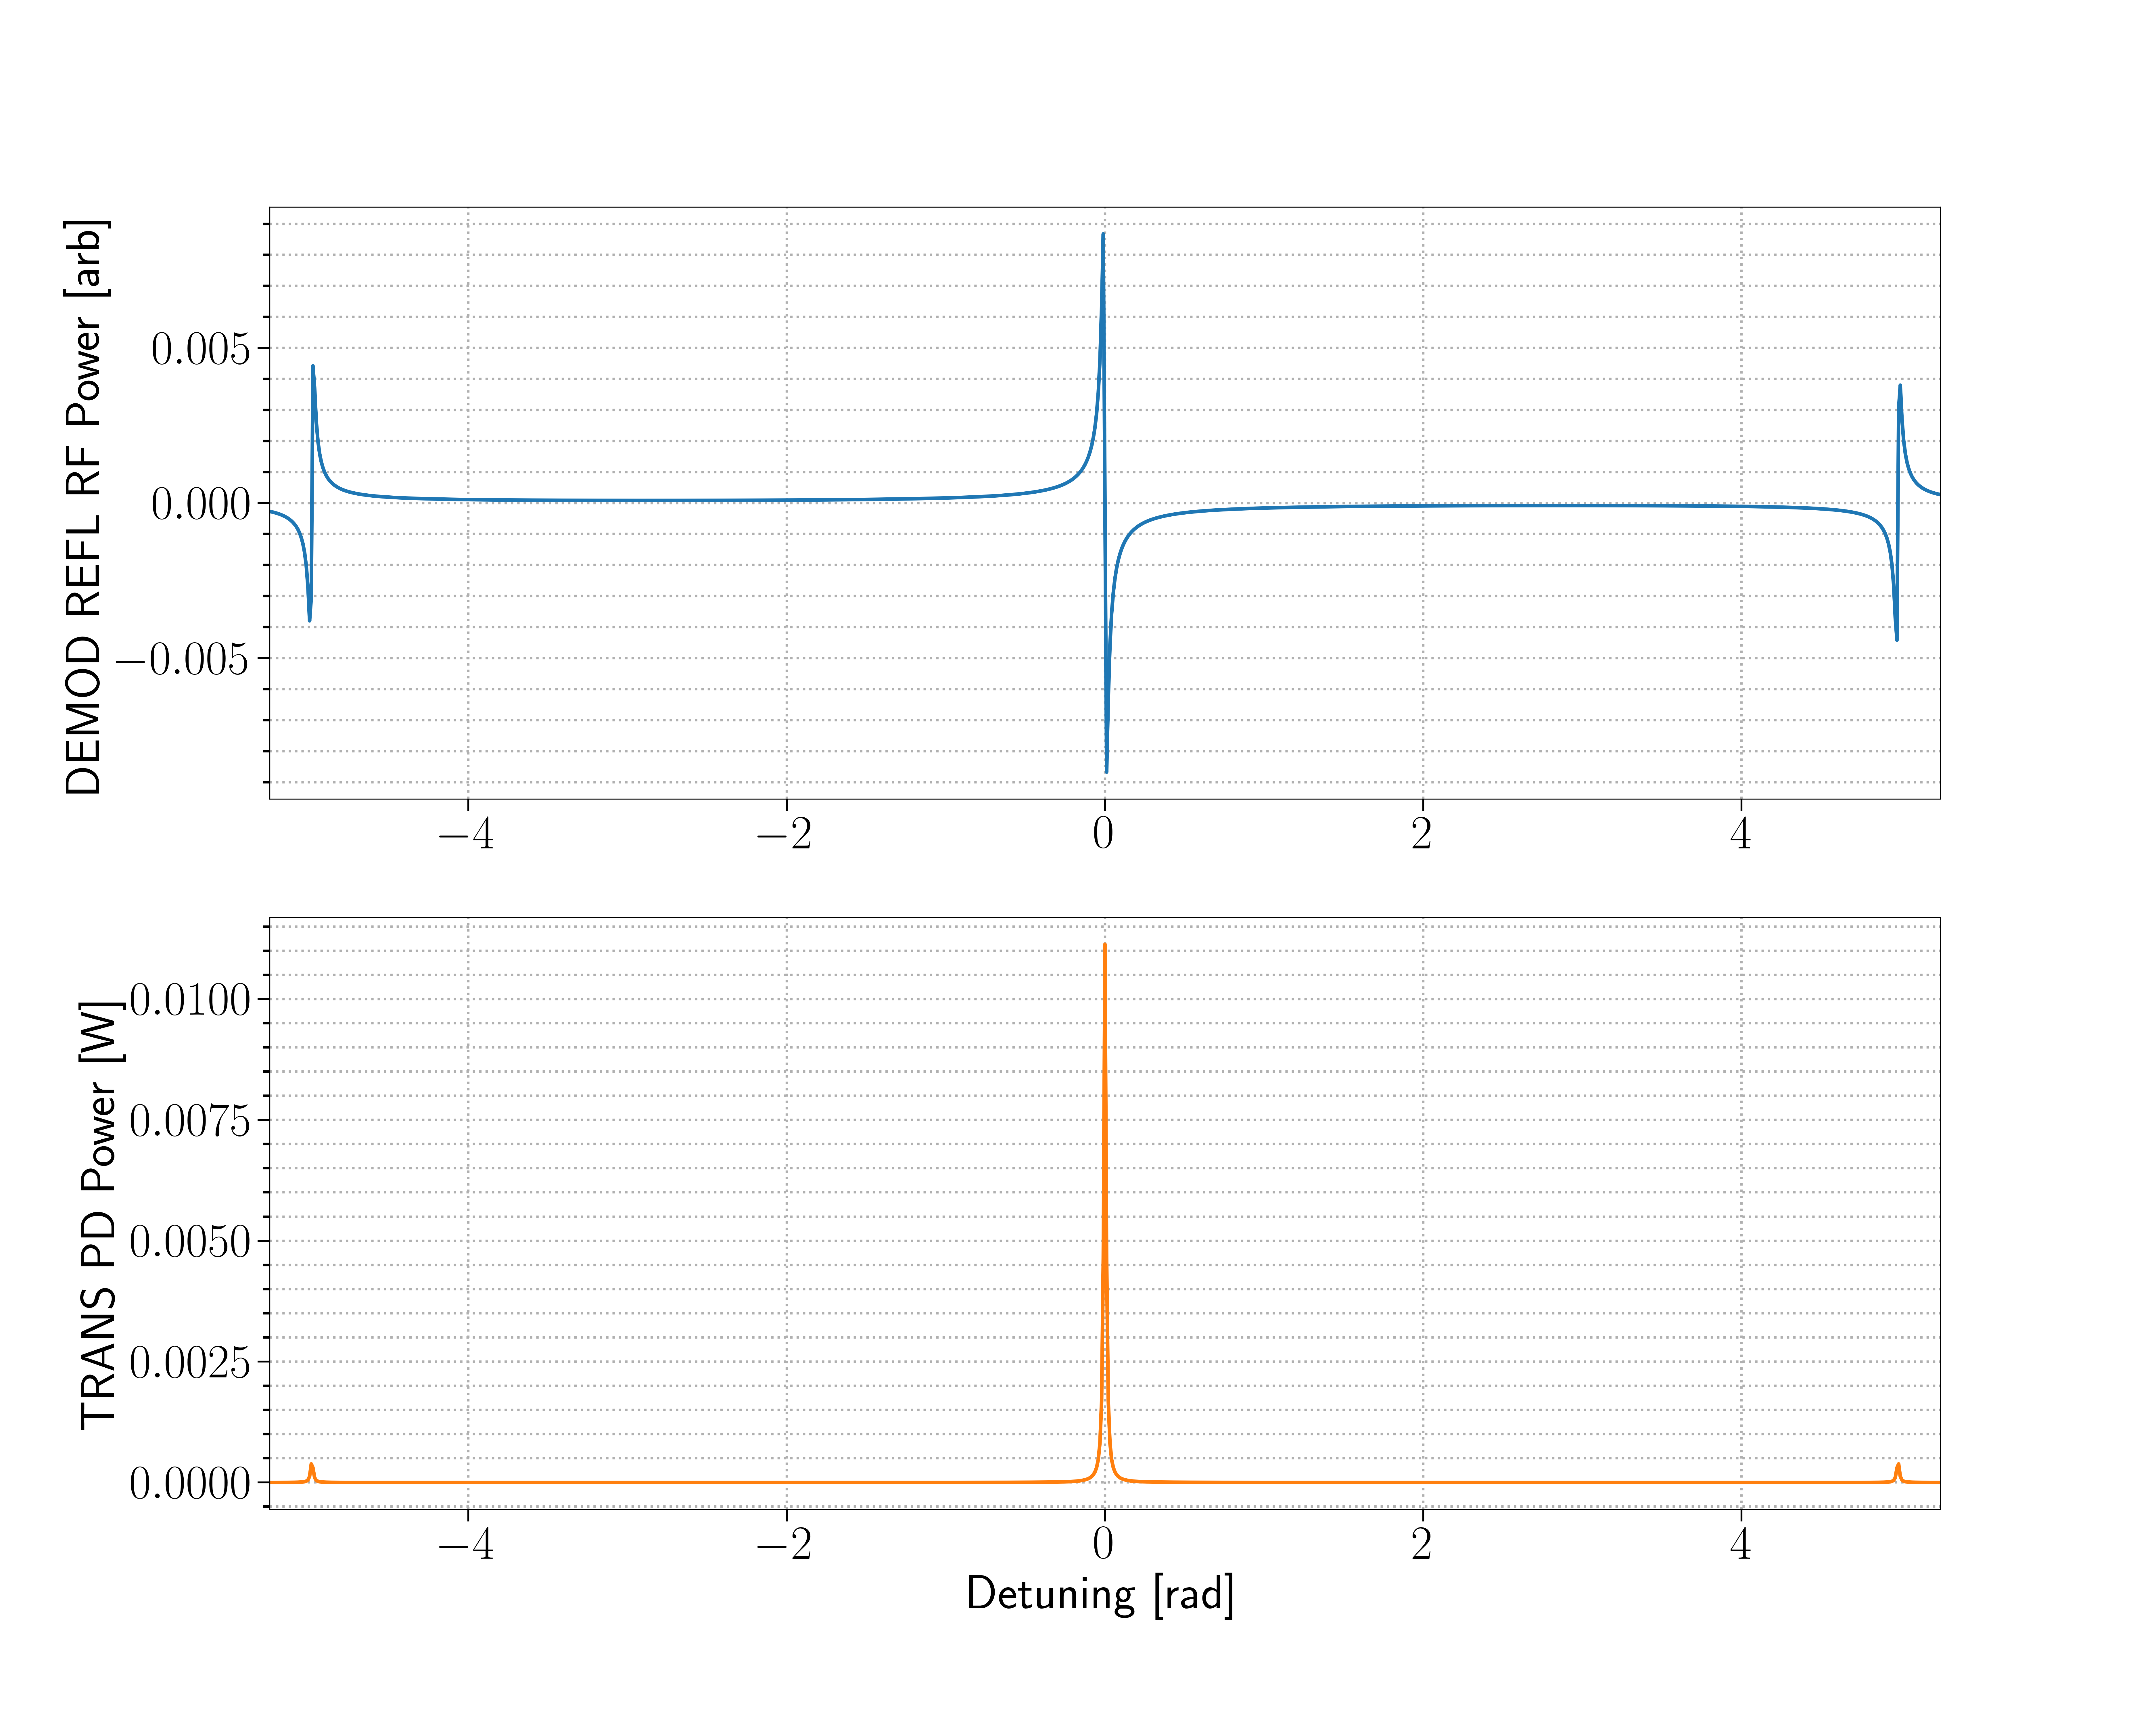
\includegraphics[width=\textwidth]{figs/ALGAAS/pdh_error.png}
\caption{By imposing 25 MHz RF sidebands we have introduced a constant reflected reference field near carrier resonance which when beat with the carrier offers a linear response after demodulating the sideband power. With the introduction of high and low frequency sideband fields, their presence is also detected through the DCPDs and PDH error signal. Their separation from resonance is equal in phase (length, and frequency) from carrier resonance.}
\label{fig:pdh_error}
\end{figure}

With this linearity and sensitivity at cavity resonance, implementation into PID feedback is the next task as any small detuning of the cavity can be registered as a drift from the loop's zero point and fed back to an actuator with an estimated calibration gain factor. When implemented into a low-noise design, this servo can also be used for a high sensitivity lock-in measurement; and with well characterized instrumentation, calibration of the induced differential phase of the light within the stable reference cavity into differential length (or frequency).


\subsection{Servo Design}
The quantity we are attempting to measure is on the order of a length change of ? m/(V/m), motivating a short cavity design as the relative differential length (phase) change scales with the sensitivity $\Delta f / f = \delta L / L$. Considerations of the lab mirror inventory and mode matching critera lead us to two candidate HR IBS coated sample (PL-CC, ROC =0.333 m) input couplers; one from CVI Melles-Griot and another from ATFilms. When paired with a GaAs/$\mathrm{Al_{.92}Ga_{.08}As}$ (PL-PL) mirror from the Crystalline Mirror Solutions (CMS) division of Thorlabs we create a 0.1665 m long cavity.

\textcolor{red}{FIGURE: Detailed optical path indicating the branching off of path mode matched to PMC}
\textcolor{red}{CAPTION: Detailed optical schema of the experiment. Components highlighted in magenta indicate laser back-reflection protection and output power control. All optics highlighted in PURPLE indicate their function as alignment and mode matching for locking to a triangular ALIGO PMC \textbf{Multiple citations (DCC doc / Fabian's experiment / Erik's experiment)}. Optics highlighted in YELLOW indicate function for alignment and mode matching experimental cavity utilizing the HR $\gaas$/$\algaas$ mirror. Beam profiling to the sample cavity is indicated. For the sake of the numerous mounting strategies tried, the longitudinal pockels cell mirror mount is kept general with the pictured mirror between two disk capacitors}
\\
\textcolor{red}{FIGURE: Servo diagram}
\textcolor{red}{caption: A simplified diagram of the servo used. The highlighted regions of the schematic are intended to provide a modular view; highlighting the components required for the PDH servo to operate.}
The implemented servo design uses a light source from a Mephisto 2000 NE Nd:YAG (1064nm) laser with a 25 MHz phase modulation from a New Focus Model 4003 IR resonant phase modulator. As indicated in the figure above, the electronics chain can be decomposed into various filter components: $S(f)$, $A(f)$, and $A_\mathrm{thermal}(f)$

\subsubsection{Sensing S(f)}
\begin{itemize}
\item 25 MHz RFPD
\begin{itemize}
\item Transimpedance measurement (necessary? or should I just use the mixer out PDH to summarize PD/mixer response)
\end{itemize}
\item Frequency Stabilization servo (modified MIT FSS (DCCD980536)) (LTspice model in appendix)
\end{itemize}


\subsubsection{Actuation A(f)}
\begin{itemize}
\item Mephisto 2220 PZT response (capacitance estimated from HVA drive measurement with and without connection to PZT)
\item Channel 3 of SVR 350-3 BIP High Voltage Amplifier from Piezomechanik GmbH with Pomona box (elog 412)
\item \textcolor{red}{Figure of frequency response of A(f)}

\end{itemize}

\subsubsection{Low frequency servo (Thermal loop)}
\begin{itemize}
\item Passed signal from FSS $\rightarrow$ integrators $\rightarrow$ Laser thermal actuator input
\end{itemize}

\subsubsection{OLG(f)}
Isn't quite $\mathrm{A}(f)*\mathrm{S}(f)$ as stated. Doesn't entirely account for the optical plant.
How the measurement is taken (important to take between installations to account for the changes in the optical plant) (elog 831)


\subsection{Longitudinal Pockels Cell mirror mount assembly}
Maximizing the electric field ($|E_z|$) and within the coating while requiring a through beam to and through the HR coating lead us to a design very similar to that of a longitudinal pockels cell \cite{}. The assembly is comprised of two disk electrodes with a 3mm central aperture which is chosen to be at least 5 times larger than the beam size at the plate locations; to avoid significant beam clipping while maximizing field strength at the coating region of interest. There is also a required separation of at least 1/4" accounting for the thickness of the optical sample. Considering these constraints, modelling the system and computing the estimated field strength screened by the coating is the next step to the construction of the assembly.

\subsubsection{Modelling}

\textcolor{red}{here (figure showing the the electrode plates, and sample with AlGaAs coating}
To find the Electric field screened by the coating we begin with Gauss' Law:

\begin{equation}
\nabla \cdot D = \rho_\mathrm{free}
\end{equation}
For our problem we assume no free charge, but the fused silica substrate with the AlGaAs coating presents dielectric material between the plates. Our initial boundary conditions are also expressed in terms of plate potentials so it is natural to first solve for the potential ($V$) for every point within our system. We can exploit the cylindrical symmetry with the optic and plate geometry in the $r$ coordinate so we shall express the Laplacian accordingly:
\begin{equation}
(1-\chi)\bigg[\frac{1}{r}\frac{\partial}{\partial r} \bigg( r \frac{\partial}{\partial r}\bigg) + \frac{\partial^2}{\partial z^2}\bigg]V = 0
\end{equation}
Where $\chi$ is a spatially dependent electric susceptibility. (\textcolor{red}{Establish coordinates for $\gaas$/$\algaas$, as well as the fused silica substrate so the computation is transparent})
\\
\satoshi{Definition of $\rho$ must be explained. $\rho$ and $\rho_{\mathrm{free}}$ are confusing.
Define $\chi$ and $V$.}

\begin{itemize}
\item Potential map computation in cylindrical
\item Computing $E_z$ from potential map
\begin{itemize}
\item inside coating
\item outside coating
\end{itemize}
\end{itemize}


\begin{figure}[H]
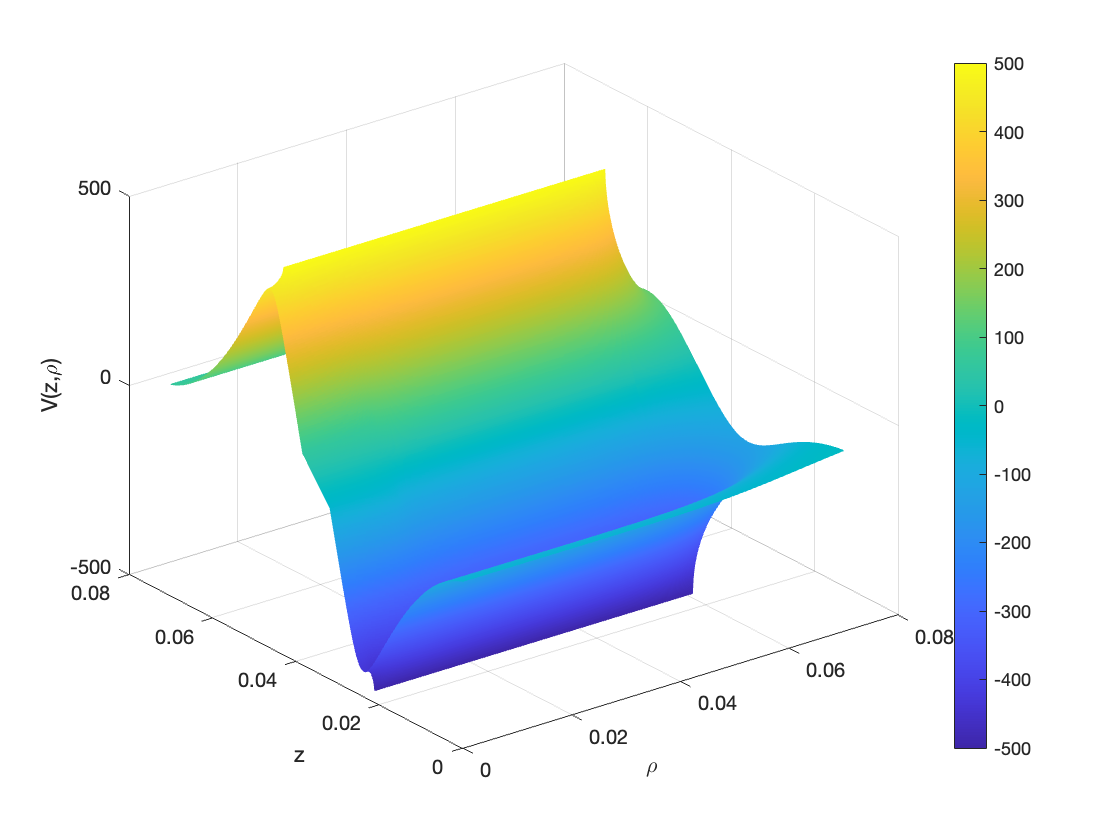
\includegraphics[width=\textwidth]{ALGAAS/13-Sep-2021_potential_map}
\caption{Poisson calculator output potential map ($V(z,r)$ in cylindrical coordinates)}
\label{fig:poisson_calc_output}
\end{figure}

\begin{figure}[H]
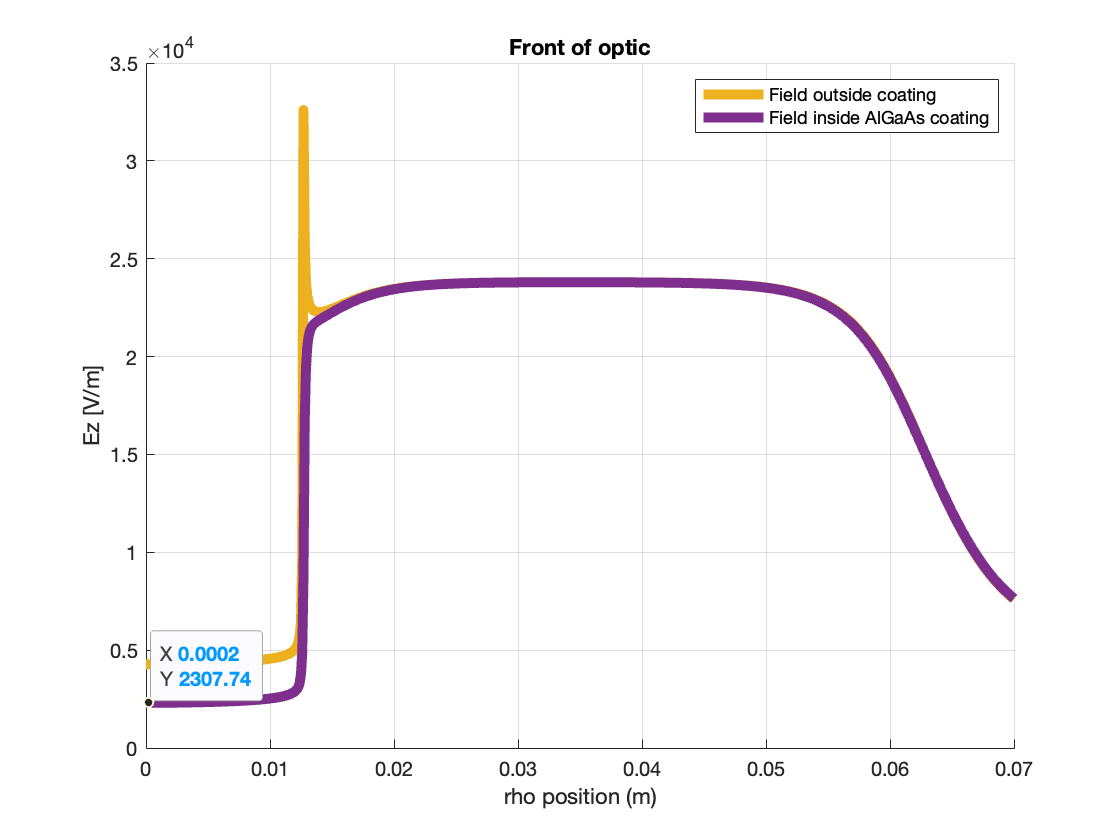
\includegraphics[width=\textwidth]{ALGAAS/13-Sep-2021_e_field_inside_outside_normal}
\caption{$|E_z|$ screened by the scoating and immediately outside AlGaAs coating. \textcolor{red}{Needs to be updated with more current settings}}

\satoshi{How large applied voltage is assumed?}

\label{fig:Ez}
\end{figure}

\begin{figure}[H]
\centering
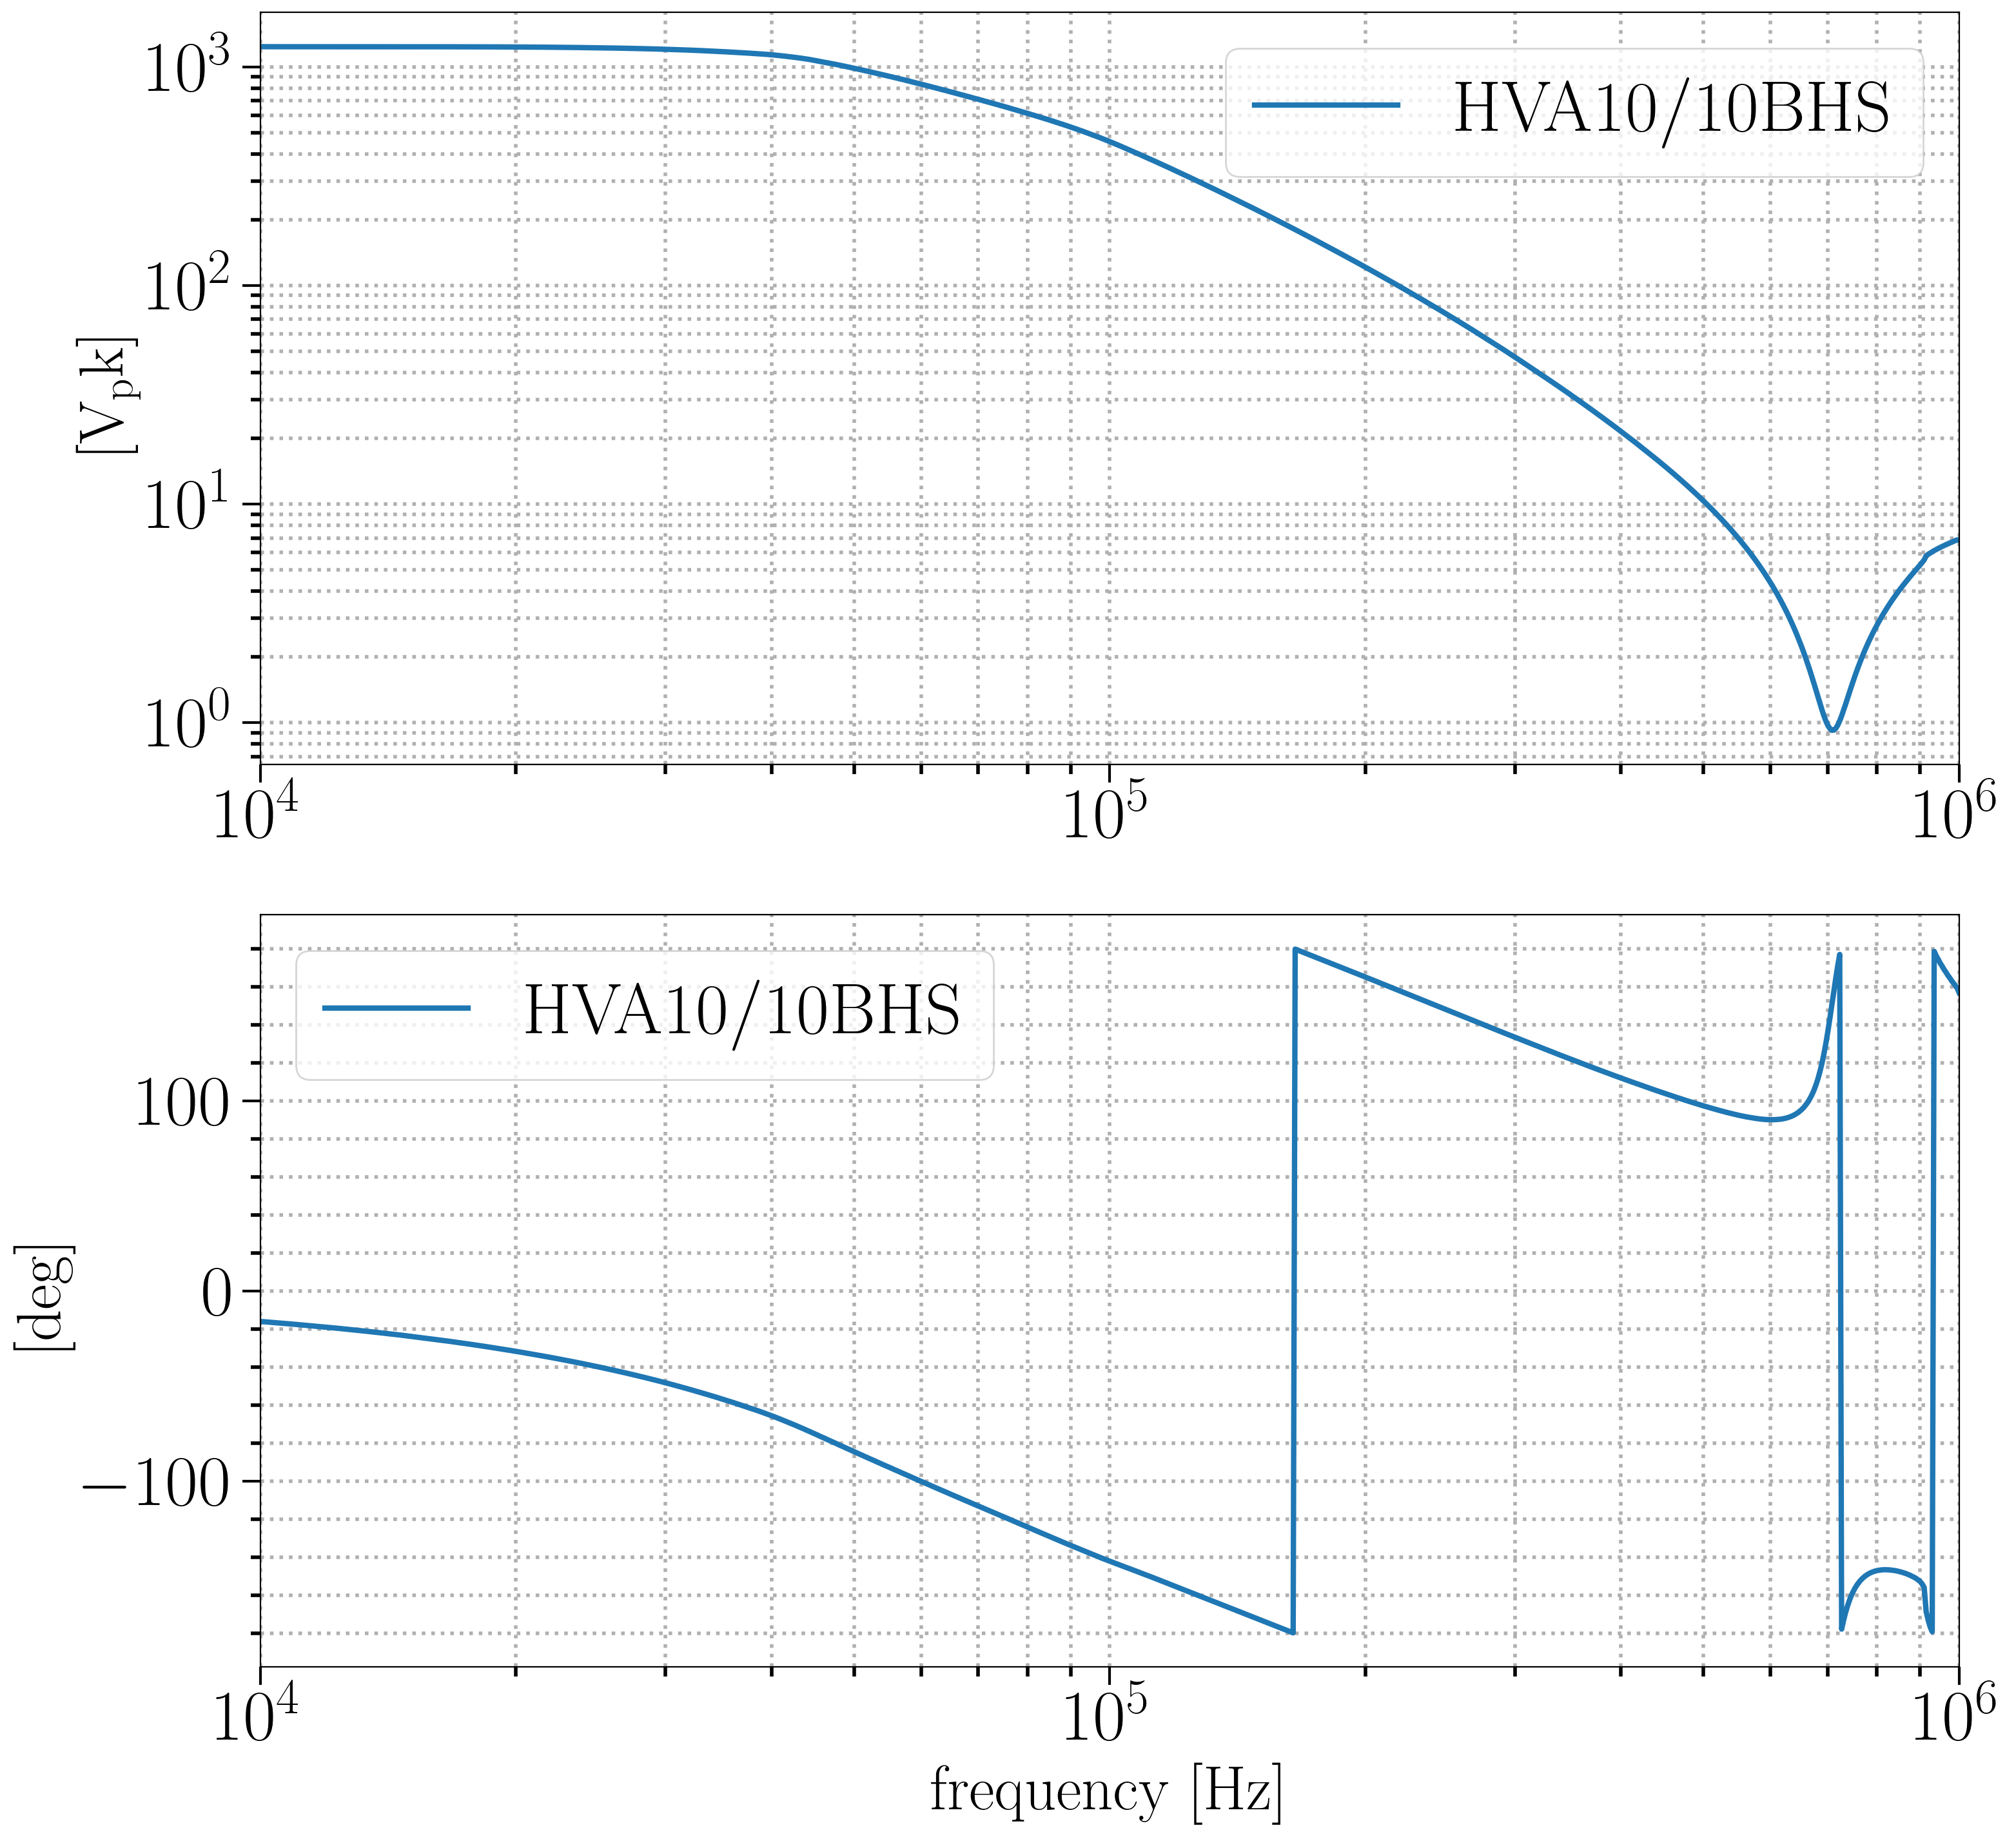
\includegraphics[width=.75\textwidth]{figs/ALGAAS/HVA_TREK1010BHS_1260V_out.png}
\caption{TREK 10/10B-HS HVA frequency dependent measurement. Using Poisson calculator to estimate field strength within coating. (\textcolor{red}{Just HVA for now but will update.} \textcolor{red}{Also, assumes a flat response from coating within this studied region (is this a good assumption or could I do better? (dielectric frequency dependence))}}
\label{fig:Ez}
\end{figure}

\subsubsection{Constructions}
Most commercial optical mounts are conductive which proved to be a problem when attempting to find a mounting solution while reducing the non-normal field gradients within the volume of interest around the sample. Because of this, we chose to construct an optical mount made of MACOR a machinable ceramic with high a high Young's modulus (66.9 GPa), and a moderate Poisson ratio (.29) \cite{macor}. An optical mount for the sample made with MACOR, along with glass bearnings .48 $\pm$ .01 cm $\diameter$  and a McMaster-Carr 8-32, 1/2" ceramic screw were used to clamp and suspend the optical sample. A 1.24" $\diameter$ hole was bored into the MACOR with a (\textcolor{red}{depth?}) depth so that there is a ? mm clearance between the front and back surface of the sample to the electrode plates.
\textcolor{red}{Figure with the sample in-situ}
\\
\begin{figure}[H]
\centering
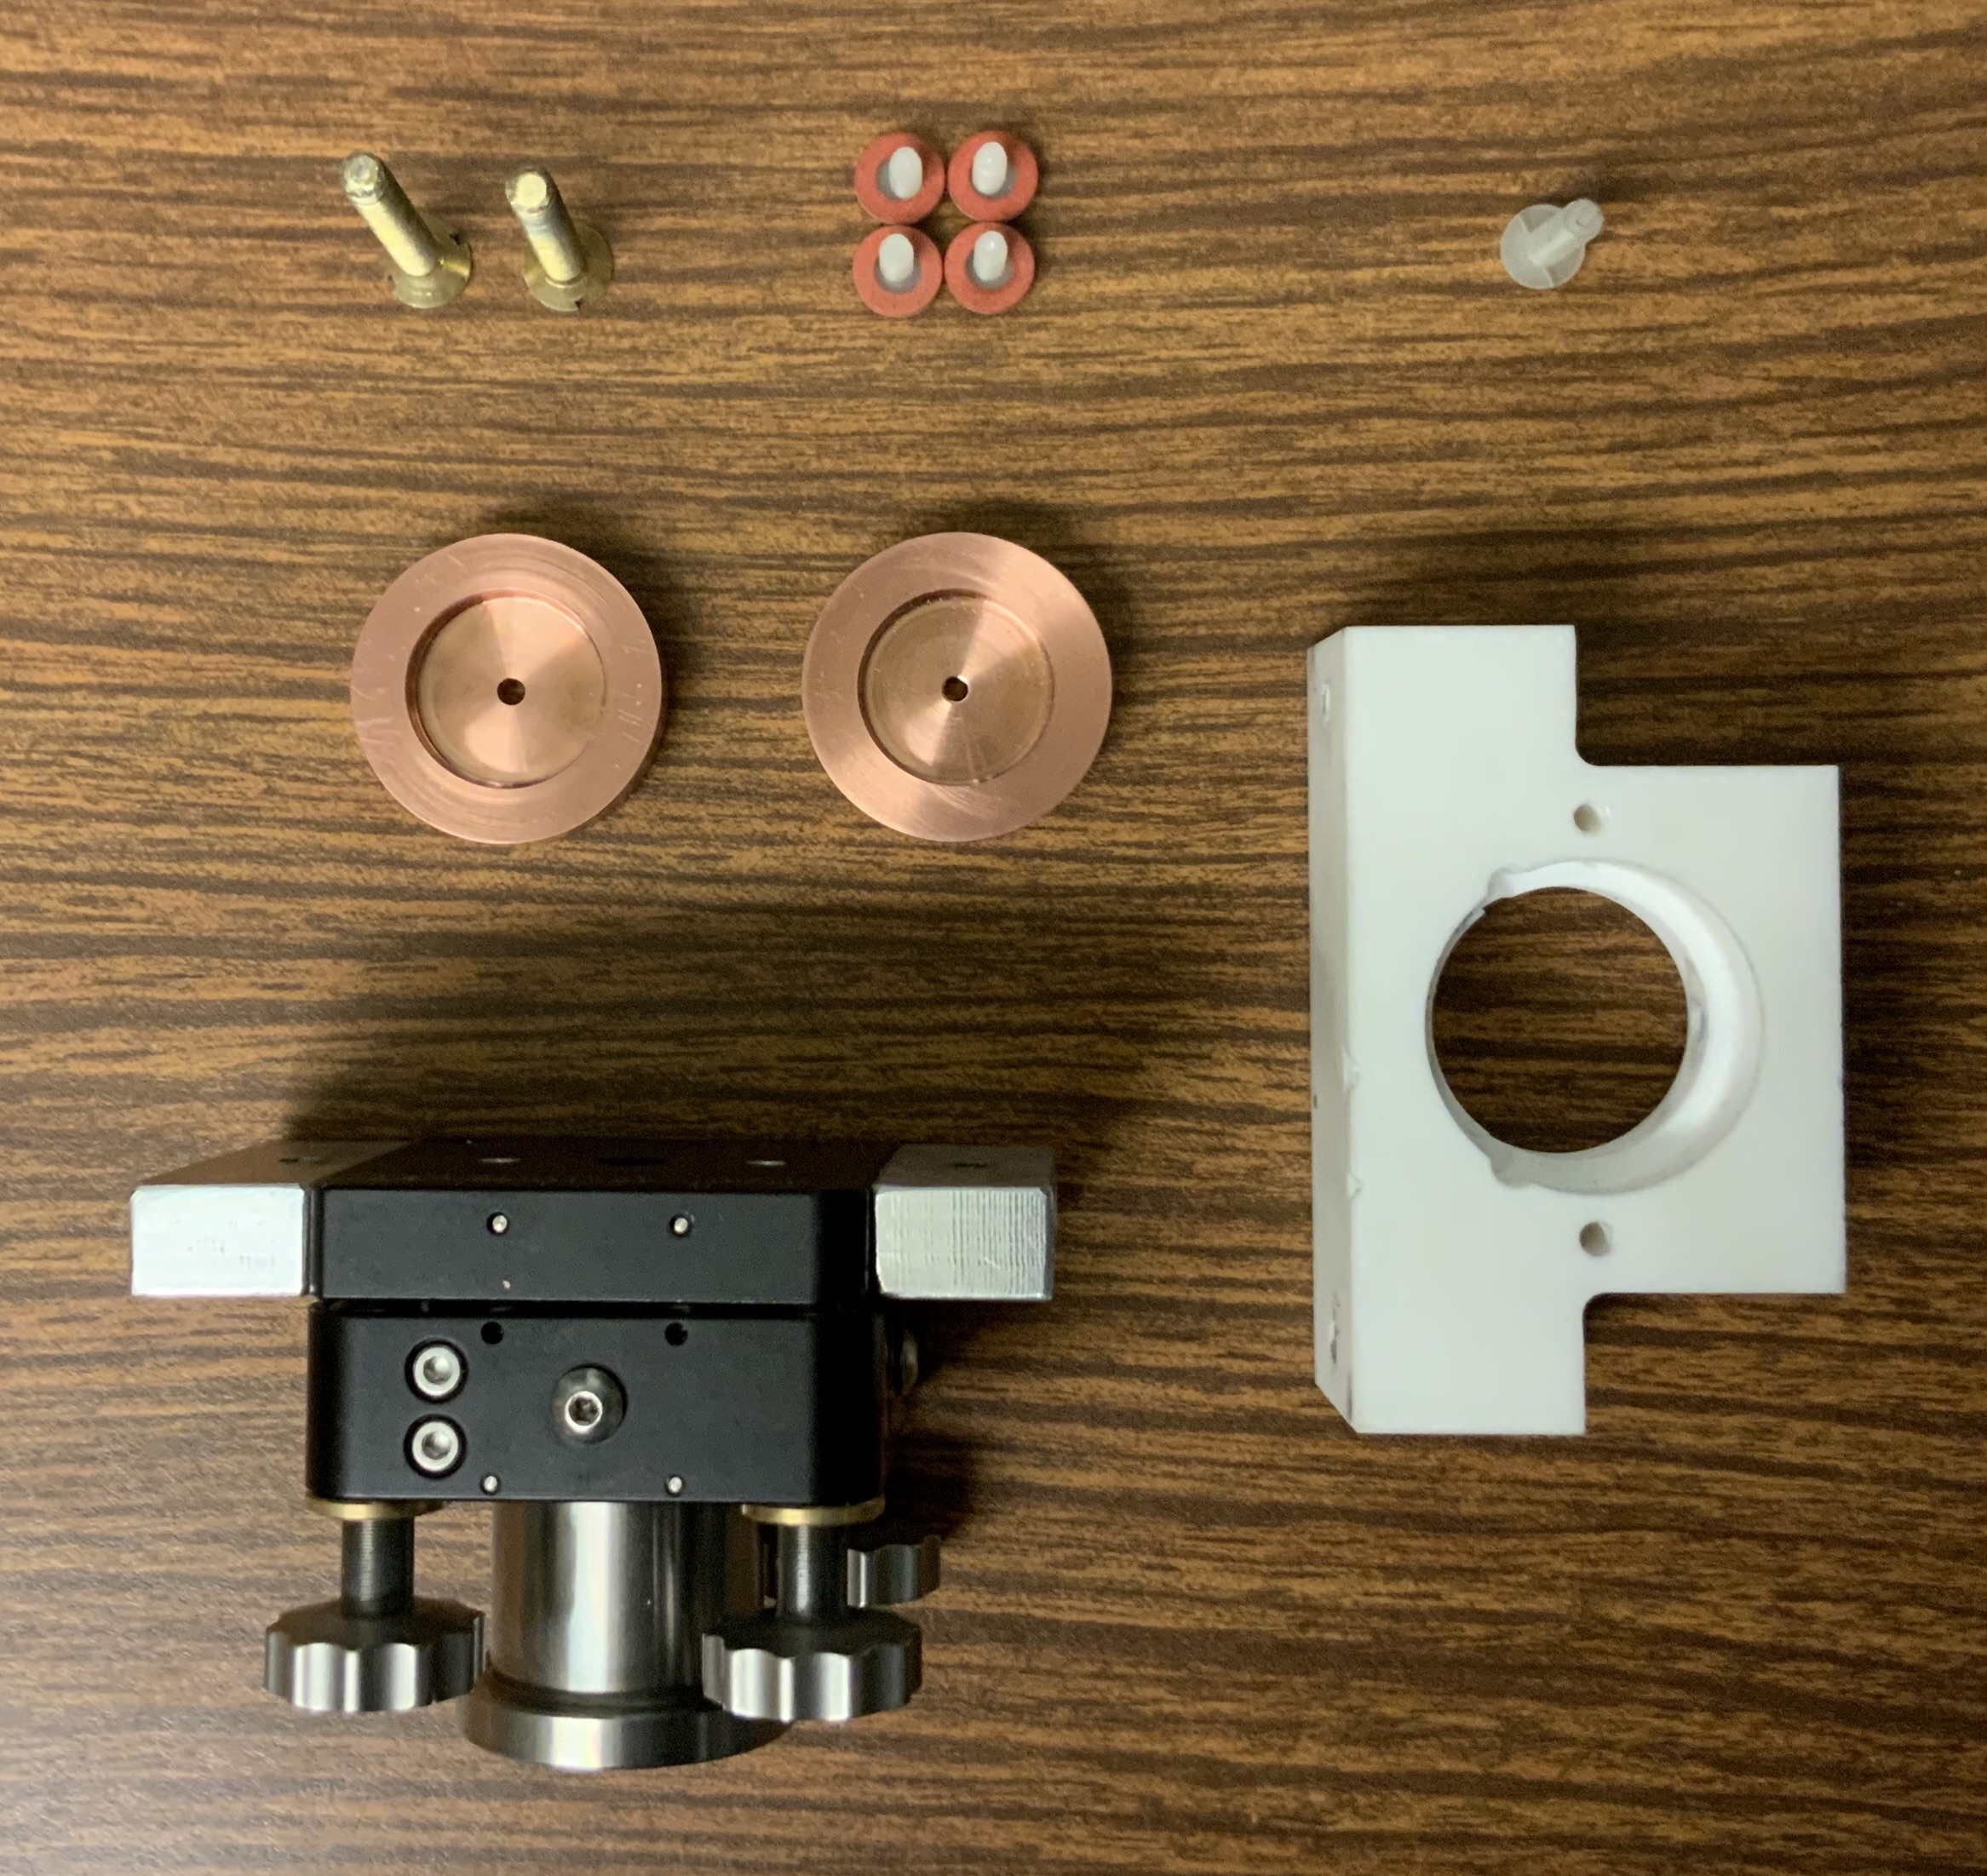
\includegraphics[width=.75\textwidth]{figs/ALGAAS/macor_assembly.jpeg}
\caption{Placeholder for more updated MACOR assembly}
\label{fig:Ez}
\end{figure}
\textcolor{red}{Review notes and list all experiment configurations. Things modified from experiment to experiment: injection / measurement type (single frequency and transfer functions (with various ranges), mounts (Differing geometries, differing materials: PLA, PETG, MACOR), electrode sizes, separations, and assembly configurations}
\subsection{Measurement Calibration}
The measurements recorded were taken with two
As discussed, we know that the error signal spectra provides us a voltage spectra that with the above information about the servo electronics, allows us to
$\mathrm{VFSSOUT}_\mathrm{rms}/\sqrt{Hz} \rightarrow m_\mathrm{rms}/\sqrt{\mathrm{Hz}}$

$$\Delta \mathrm{L} = \mathrm{source}*\alpha(f) \mathrm{A}(f)*\frac{1+\mathrm{OLG}(f)}{\mathrm{OLG}(f)}*\frac{\mathrm{L_{cav}}}{f_\mathrm{laser}}$$

\subsection{Noise Floor}

%\begin{itemize}
%\item Measure with initial LIGO PMC?
%\item There is also a spectra in the Mephisto laser spec sheets
%\end{itemize}

\subsection{Results}

\subsubsection{Mount noise (3D printed mount mechanical noise)}
Various mount designs were designed / prototyped.

\subsubsection{Drive coupling}

\begin{figure}[H]
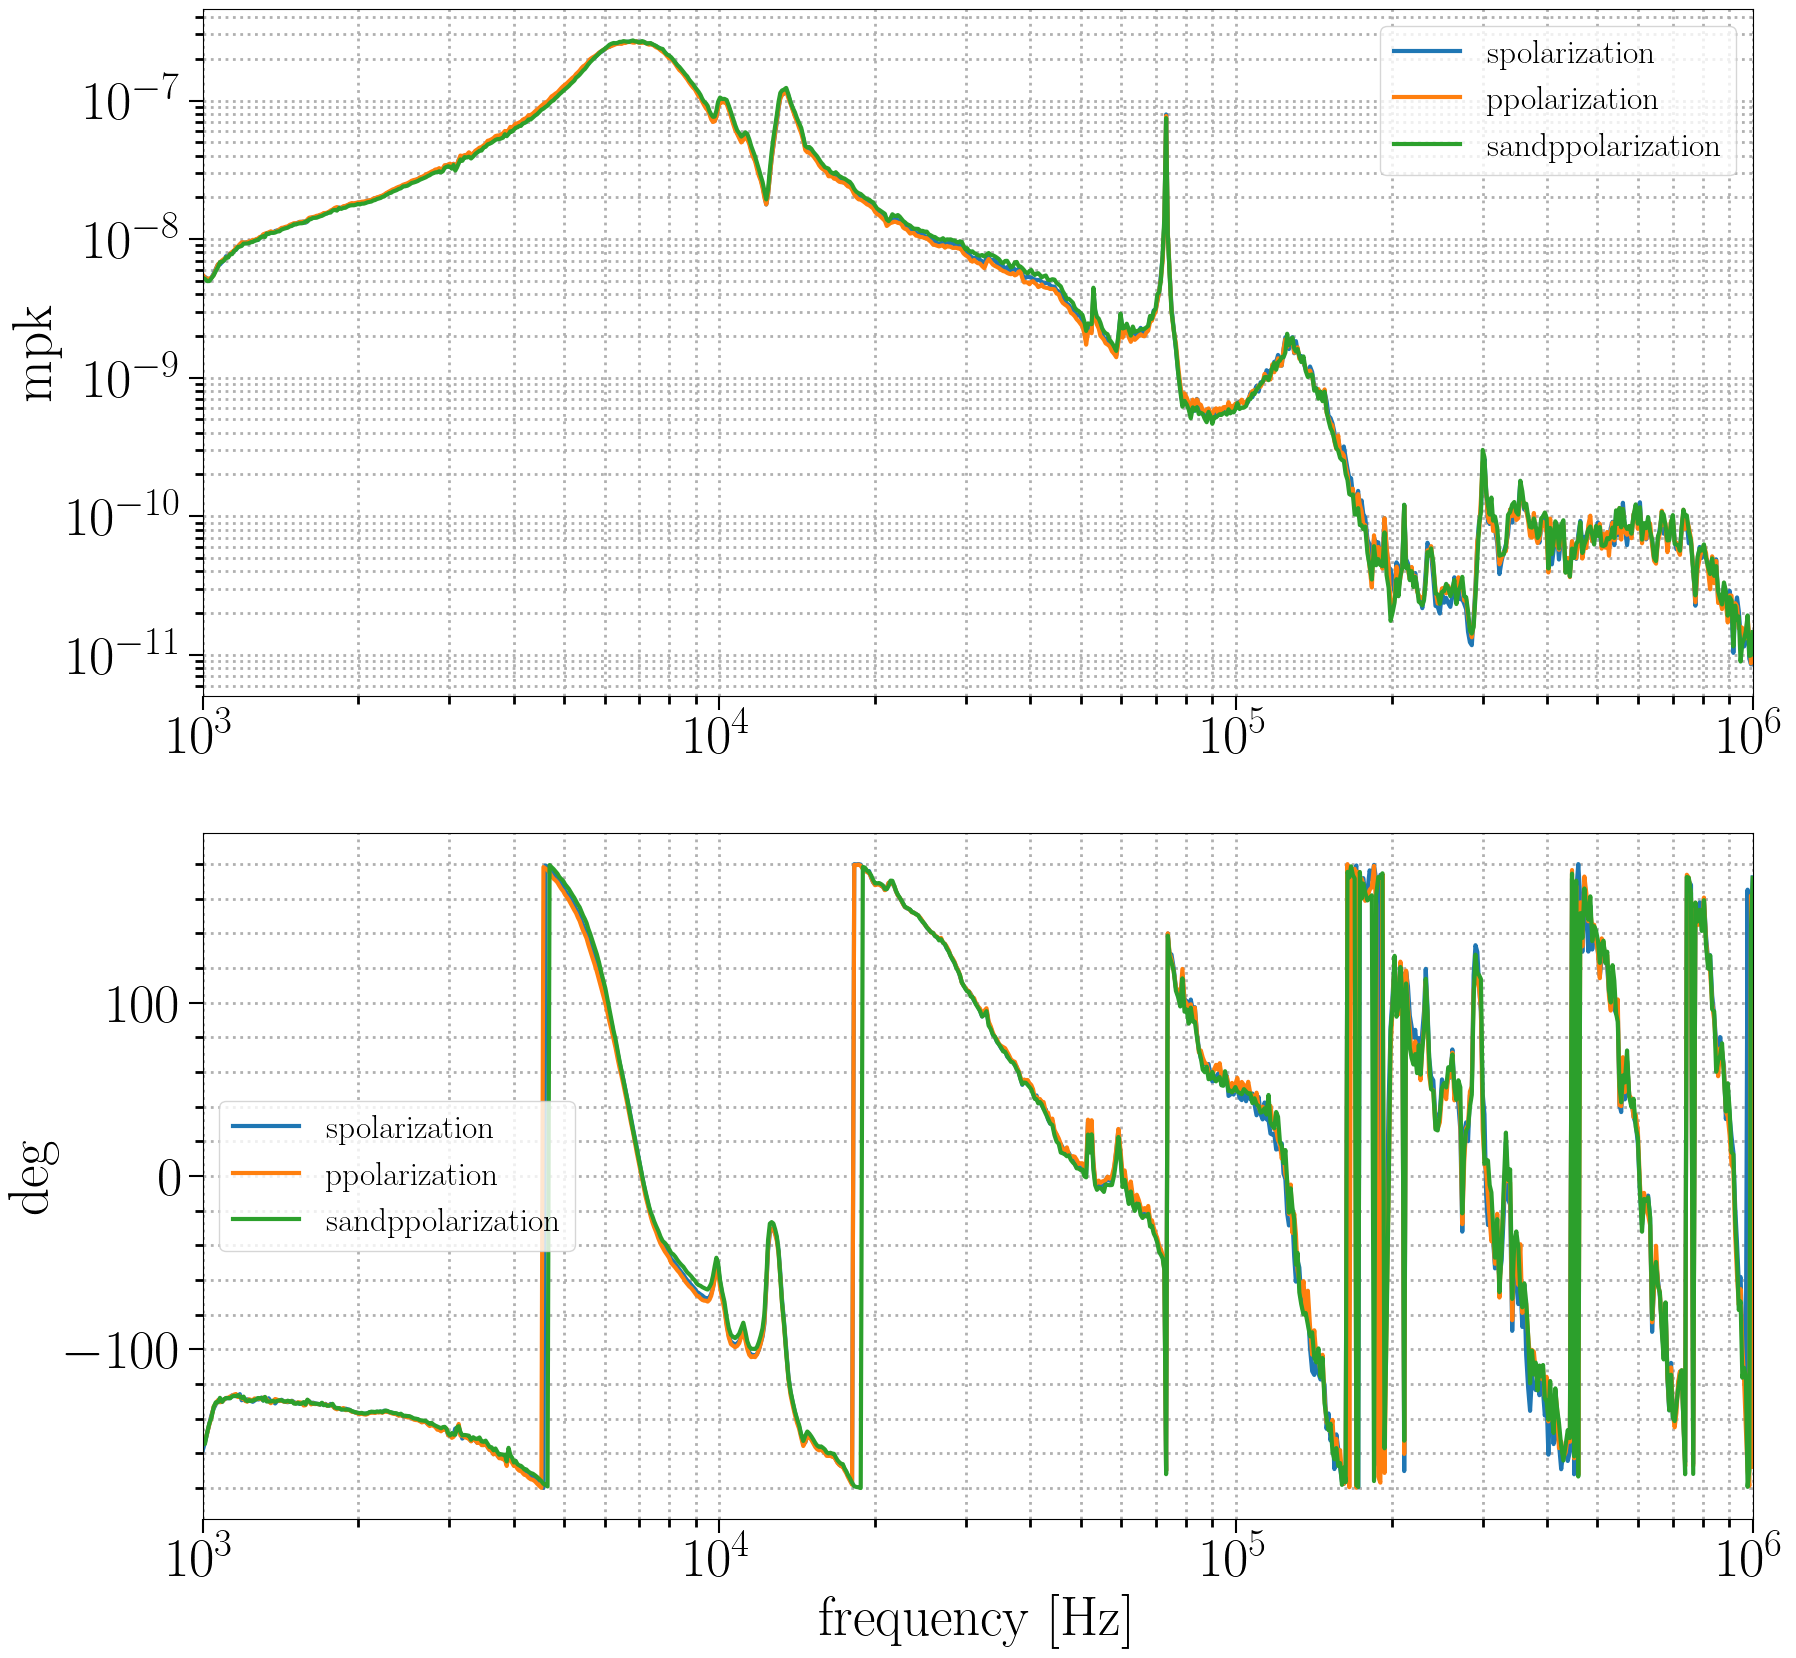
\includegraphics[width=\textwidth]{figs/ALGAAS/cav_polarization_test.png}
\caption{Figure that will include the displacement noise floor, (pockels estimate)*(poisson calculator estimate)*(HVA drive frequency dependence), and the drive coupled measurement \textcolor{red}{figure size needs to be increased}}
\label{fig:measurement_sum}
\end{figure}

\subsubsection{Opto-mechanical coupling}
Sample and mount mechanical mode excitations. Seen with both AlGaAs and a HR coating from an AtFilm (IBS coating)
\begin{itemize}
\item \textbf{Vibration of plates (Leissa)} \cite{leissa} Computing frequencies and order of magnitude
\item \textbf{Steve's COMSOL model results}
\end{itemize}

\subsubsection{Dual-polarization locked}
